% ============================================================================
% LA GÉOMÉTRIE DU SPECTRE DES NOMBRES PREMIERS
% Avec validations formelles Isabelle/HOL COMPLÈTES ET EXACTES
% Auteur : Philippe Thomas Savard
% Version française
% ============================================================================

\documentclass[a4paper,11pt]{article}

% ============================================================================
% PACKAGES
% ============================================================================
\usepackage[utf8]{inputenc}
\usepackage[T1]{fontenc}
\usepackage[french]{babel}
\usepackage{amsmath,amssymb,amsthm}
\usepackage{mathtools}
\usepackage{graphicx}
\graphicspath{{images/}{./images/}}
\usepackage{float}
\usepackage{booktabs}
\usepackage{array}
\usepackage{longtable}
\usepackage{multirow}
\usepackage{geometry}
\usepackage{fancyhdr}
\usepackage{titlesec}
\usepackage{tocloft}
\usepackage{xcolor}
\usepackage{listings}
\usepackage{listingsutf8}
\usepackage{tcolorbox}
\usepackage{enumitem}
\usepackage{caption}
\usepackage{hyperref} % hyperref doit être chargé en dernier

% ============================================================================
% CONFIGURATION DE LA PAGE
% ============================================================================
\geometry{margin=2.5cm}

% Configuration de la table des matières
\setcounter{tocdepth}{3}
\setcounter{secnumdepth}{3}

% Configuration des couleurs
\definecolor{holblue}{RGB}{0,102,153}
\definecolor{holgreen}{RGB}{0,128,0}
\definecolor{holpurple}{RGB}{102,0,153}
\definecolor{lightgray}{RGB}{245,245,245}
\definecolor{darkgray}{RGB}{50,50,50}

% Configuration des hyperliens
\hypersetup{
    colorlinks=true,
    linkcolor=holblue,
    urlcolor=holblue,
    citecolor=holblue
}

% ============================================================================
% CONFIGURATION LISTINGS POUR CODE HOL
% ============================================================================
\lstdefinelanguage{isabelle}{
  keywords={theory, imports, begin, end, definition, where, fun, lemma, theorem, proof, qed, shows, assumes, fixes, and, if, then, else, let, in, axiomatization, section, subsection, text},
  keywordstyle=\color{holblue}\bfseries,
  sensitive=true,
  morecomment=[l]{--},
  morecomment=[s]{(*}{*)},
  commentstyle=\color{holgreen}\itshape,
  stringstyle=\color{holpurple},
  morestring=[b]",
  literate=
           {λ}{{$\lambda$}}1 
           {→}{{$\rightarrow$}}1 
           {⟶}{{$\longrightarrow$}}1
           {⟹}{{$\Longrightarrow$}}1 
           {↔}{{$\leftrightarrow$}}1
           {∧}{{$\wedge$}}1 
           {∨}{{$\vee$}}1 
           {¬}{{$\neg$}}1
           {≤}{{$\leq$}}1 
           {≥}{{$\geq$}}1 
           {≠}{{$\neq$}}1
           {∈}{{$\in$}}1 
           {∀}{{$\forall$}}1 
           {∃}{{$\exists$}}1
           {⟷}{{$\longleftrightarrow$}}1
           {‹}{{$\langle$}}1 
           {›}{{$\rangle$}}1
           {⋀}{{$\bigwedge$}}1
           {⇒}{{$\Rightarrow$}}1
           {×}{{$\times$}}1
           {«}{{<<}}1
           {»}{{>>}}1
           {—}{{---}}1
           {é}{{\'e}}1 
           {è}{{\`e}}1 
           {ê}{{\^e}}1 
           {ë}{{\"e}}1
           {à}{{\`a}}1 
           {â}{{\^a}}1 
           {ä}{{\"a}}1
           {ù}{{\`u}}1 
           {û}{{\^u}}1 
           {ü}{{\"u}}1
           {ô}{{\^o}}1 
           {î}{{\^i}}1 
           {ï}{{\"i}}1
           {ç}{{\c{c}}}1
           {É}{{\'E}}1 
           {È}{{\`E}}1 
           {Ê}{{\^E}}1
           {À}{{\`A}}1 
           {Ô}{{\^O}}1
           {–}{{--}}1
           {'}{{`}}1
           {'}{{`}}1
           {"}{{``}}1
           {"}{{''}}1
}

\lstset{
  language=isabelle,
  basicstyle=\small\ttfamily,
  breaklines=true,
  breakatwhitespace=true,
  columns=flexible,
  keepspaces=true,
  showstringspaces=false,
  frame=none,
  backgroundcolor=\color{lightgray},
  xleftmargin=0.5cm,
  xrightmargin=0.5cm,
  inputencoding=utf8,
  extendedchars=true,
}

% ============================================================================
% ENVIRONNEMENTS PERSONNALISÉS
% ============================================================================
\tcbuselibrary{listings,skins,breakable}

\newtcolorbox{holcode}[1][]{
    enhanced,
    breakable,
    colback=lightgray,
    colframe=holblue,
    fonttitle=\bfseries,
    title={\textcolor{white}{Validation Isabelle/HOL}},
    coltitle=white,
    attach boxed title to top left={xshift=5mm,yshift=-2mm},
    boxed title style={colback=holblue},
    left=2mm,
    right=2mm,
    #1
}

\newenvironment{mydef}[1]{%
    \begin{tcolorbox}[colback=blue!5,colframe=holblue,title={\textbf{Définition : #1}}]
}{%
    \end{tcolorbox}
}

\newenvironment{exemple}[1][]{%
    \begin{tcolorbox}[colback=green!5,colframe=holgreen,title={\textbf{Exemple #1}}]
}{%
    \end{tcolorbox}
}

\newenvironment{resume}{%
    \begin{tcolorbox}[colback=purple!5,colframe=holpurple,title={\textbf{Résumé visuel}}]
}{%
    \end{tcolorbox}
}

% ============================================================================
% TITRE ET AUTEUR
% ============================================================================

\title{
    \vspace{-2cm}
    {\LARGE \textbf{La Géométrie du Spectre}}\\[0.5cm]
    {\LARGE \textbf{des Nombres Premiers}}\\[1cm]
    {\large Avec validations formelles Isabelle/HOL}\\[0.5cm]
    \rule{\textwidth}{0.4pt}
}

\author{
    \textbf{Philippe Thomas Savard}\\[0.3cm]
    \small Lévis, Chaudière-Appalaches, Québec, Canada\\
    \small 5354 rue du Menuet, Lévis, Québec, G6X 2Y6\\
    \small Téléphone : 418-487-8798
}

\date{
    \vspace{0.5cm}
    Date originale : 22 mars 2026\\
    Révision : 18 janvier 2026\\
    Compilation HOL : Mars 2026
}

% ============================================================================
% DÉBUT DU DOCUMENT
% ============================================================================
\begin{document}

\maketitle
\thispagestyle{empty}

\vspace{1cm}

\begin{abstract}
Ce document présente la \textbf{géométrie du spectre des nombres premiers}, une méthode originale développée par Philippe Thomas Savard pour étudier la distribution des nombres premiers. L'approche combine des suites fractionnaires, des rapports triangulaires et une analyse numérique métrique inspirée de la granulométrie. Toutes les démonstrations mathématiques sont accompagnées de leurs \textbf{validations formelles en Isabelle/HOL}, garantissant la rigueur logique des résultats présentés.
\end{abstract}

\newpage
\tableofcontents
\newpage

% ============================================================================
% SECTION 1 : INTRODUCTION
% ============================================================================
\section{Introduction et Déclaration de l'Auteur}

\subsection{Coordonnées de l'auteur}

\begin{center}
\begin{tabular}{ll}
\textbf{Lieu :} & Lévis, Chaudière-Appalaches \\
\textbf{Adresse :} & 5354 rue du Menuet, Lévis, Québec, Canada, G6X 2Y6 \\
\textbf{Téléphone :} & 418-487-8798 \\
\end{tabular}
\end{center}

\vspace{0.5cm}

Ce document a été rédigé sans financement, sans avantages matériels ou symboliques, et dans une totale liberté de conscience et de jugement. Ce texte est le fruit d'une expérience de pensée, illustrée par des calculs mathématiques, des schémas, des tableaux, ainsi que des exemples et explications. L'auteur n'est pas initié aux mathématiques au sens académique : il ne possède aucune formation spécialisée dans ce domaine. Il est ouvrier, et c'est en dehors des sentiers balisés qu'il a conçu ce document par pur plaisir intellectuel et en conséquence d'un intérêt profond pour les mathématiques.

\subsection{Un mot de l'auteur}

Le document que vous vous apprêtez à lire s'inscrit dans une quête quotidienne, intime et persistante, qui habite l'auteur depuis toujours. Une quête qui, probablement, ne le quittera jamais.

\begin{resume}
\textbf{Imaginez} un jeune élève fasciné par une propriété simple mais intrigante : entre deux nombres entiers consécutifs, il ne peut jamais y avoir moins qu'une unité. Cette observation élémentaire, enseignée dès l'école primaire, éveilla une profonde curiosité qui mena, des années plus tard, à la découverte présentée dans ce document.
\end{resume}

Très jeune, l'auteur s'intéressa à la distribution des nombres entiers. Il tenta une expérience naïve mais révélatrice : ajouter successivement la valeur de 1 unité à des nombres pairs. Par exemple :
\begin{itemize}
    \item $1 + 50 = 51$
    \item $1 + 100 = 101$
    \item $1 + 200 = 201$
    \item $1 + 800 = 801$
\end{itemize}

Il observa que les rapports entre ces ajouts donnaient tous $\frac{1}{2}$, lorsque mis en relation les valeurs ajoutés sont comparés pour leurs rapports entre eux? :
\[
\frac{50}{100} = \frac{100}{200} = \frac{200}{400} = \frac{400}{800} = \frac{1}{2}
\]

\begin{resume}
\textbf{Visualisez} cette decouverte comme une echelle dont chaque barreau se situe exactement a mi-chemin entre le precedent et le suivant. Cette fraction constante, 1/2, agit alors comme un fil conducteur reliant l'ensemble des nombres entiers.
\end{resume}

Plus tard, au debut du secondaire, l'auteur decouvrit les nombres premiers. Un nombre premier est un entier divisible uniquement par 1 et par lui-meme. Les dix premiers nombres premiers sont : 2, 3, 5, 7, 11, 13, 17, 19, 23 et 29.

Ce petit exercice de jeunesse, qui lui avait permis d'entrevoir l'existence d'un rapport inferieur a l'unite entre deux entiers, lui revint en memoire lorsqu'il appliqua la meme idee a une question nee de sa curiosite pour les mathematiques. Cette question, qu'il decouvrit par hasard au fil de ses lectures, etait celle de l'hypothese de Riemann. Il en fut immediatement fascine, se rappelant l'experience intuitive qu'il avait elaboree dans son enfance.

Apres avoir termine la lecture de l'article consacre a Bernhard Riemann, il se demanda si cette enigme meritait reellement l'attention que l'on lui porte. Cette interrogation le poussa a reflechir plus profondement. Il constata que les zeros non triviaux de la fonction zeta de Riemann — au coeur meme de l'hypothese — sont presents en quantite infinie. Puisque ces zeros determinent la repartition des nombres premiers, il lui sembla naturel que les parties reelles auxquelles l'hypothese fait reference ne puissent etre en nombre inferieur a cette infinite de zeros.

C'est ainsi qu'il mit au point une methode, la \emph{methode de Philippot}, sujet central du present document et dont une validation formelle via Isabelle est egalement incluse. Cette methode fut concue pour que les operations iteratives, identiques d'une etape a l'autre, permettent de determiner une infinite de fois le rapport 1/2. S'il parvenait a demontrer qu'il est impossible d'obtenir cette infinite de valeurs, alors, par l'absurde, il infirmerait l'hypothese de Riemann : en effet, les parties reelles ne sauraient etre presentes en quantite moindre que les zeros non triviaux auxquels elles sont liees.

\begin{center}
\fbox{\parbox{0.8\textwidth}{
\textbf{L'énigme de Bernhard Riemann :}\\
« Est-ce que tous les zéros non triviaux de la fonction zêta de Bernhard Riemann ont tous pour partie réelle $\frac{1}{2}$ ? »
}}
\end{center}

% ============================================================================
% SECTION 2 : PREMIÈRE PARTIE - GÉOMÉTRIE DU SPECTRE
% ============================================================================
\newpage
\section{Première Partie : La Géométrie du Spectre des Nombres Premiers}

\begin{figure}[H]
    \centering
    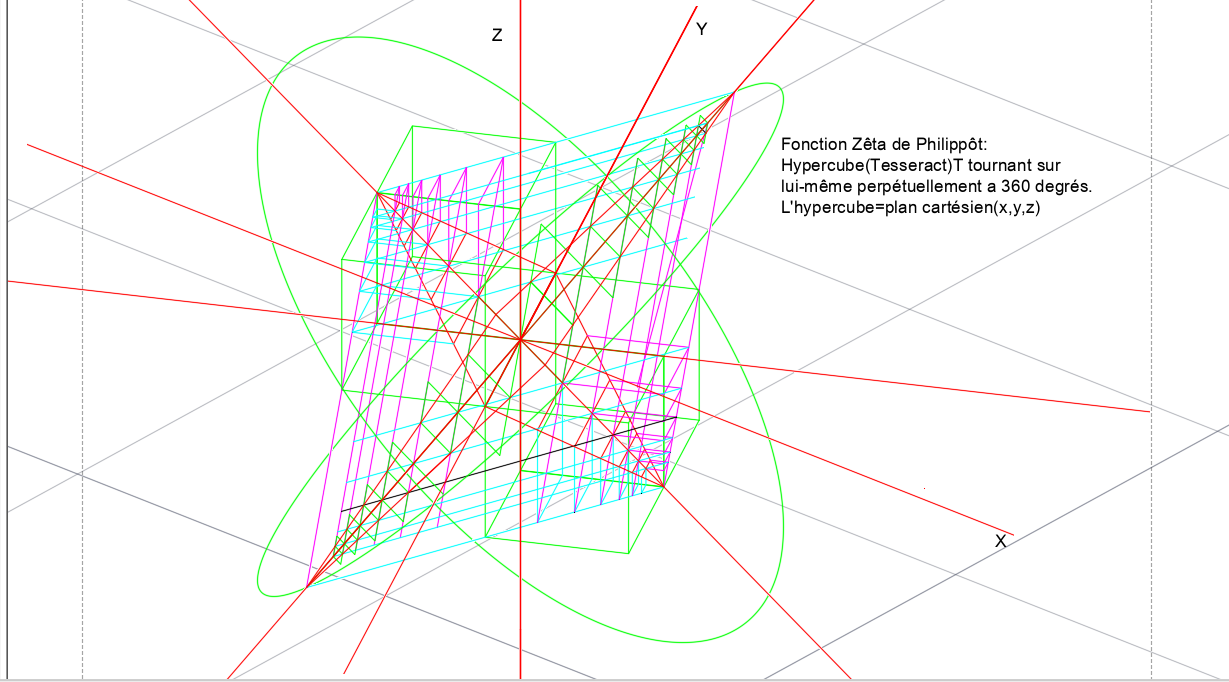
\includegraphics[width=0.9\textwidth]{fonction_zeta_riemann_philippot.png}
    \caption{Représentation de la fonction Zêta de Philippôt dans un plan $(x, y, z)$ -- L'hypercube (Tesseract) tourne sur lui-même perpétuellement à 360 degrés.}
    \label{fig:zeta}
\end{figure}

\begin{resume}
\textbf{Imaginez} la figure de la fonction Zeta de Philippot presente ci-dessus. Il s'agit d'une representation graphique composee de plusieurs sections distinctes. La premiere section remarquable est formee des quatre cubes de couleur verte. Ces quatre cubes constituent en realite un seul volume, traverse par un losange rouge selon un angle diedre. Autour de ce volume central se trouvent quatre pyramides, en mauve et en turquoise, orientees dans quatre directions opposees : vers la gauche, la droite, le haut et le bas. Chaque orientation est legerement decalee par rapport a la face avant et a la face arriere des cubes. Ces pyramides sont elles-memes composees d'une serie de carres correspondant a des divisions situees a des positions precises.

L'origine de la fonction se trouve au centre des trois axes (x, y, z). En poursuivant l'observation de l'illustration, on remarque une zone quadrillee, egalement en mauve et en turquoise. Ce maillage traverse diagonalement les quatre cubes en passant par leur diametre lateral. Cette section correspond a l'endroit exact ou se situe l'analyse numerique metrique. Nous verrons dans ce document que les nombres premiers associes aux rapports spectraux sont determines a l'aide de deux suites, appelees A et B. La quantite de termes dans chacune de ces suites determine la position du nombre premier pour le rapport spectral 1/2. Ce rapport apparaitra de maniere explicite dans la suite du document, qui inclut une validation generalisee a l'ensemble des nombres premiers P.

Pour determiner l'ensemble des nombres premiers et demontrer le rapport spectral commun, une suite d'operations doit etre appliquee. Les differents carres inclus dans les pyramides jouent le role de matrices de convolution. Les suites A et B sont definies ainsi : pour le premier nombre premier, soit 2, la suite contient un terme; pour le deuxieme, 3, elle contient deux termes; pour le troisieme, 5, trois termes; et ainsi de suite. Le meme principe s'applique aux nombres premiers negatifs : pour -2, il y a -1 terme; pour -3, -2 termes; pour -5, -3 termes, etc. Cette affirmation est validee pour le rapport 1/2. Les autres rapports spectraux presentent quelques variations, et deux exemples sont fournis et detailles dans la validation formalisee et generalisee a l'ensemble des nombres premiers par Isabelle, incluse dans ce document.

Nous disions que les carres inclus dans les pyramides servent de matrices pour une serie de convolutions. Les resultats de ces convolutions sont obtenus par projection orthogonale d'un hypercube sur une surface quadrillee. Ces convolutions suivent le rythme de la rotation et du repli de l'hypercube, qui se replie sur lui-meme tout en tournant, permettant ainsi la projection orthogonale sur la surface. Sur cette surface, on observe une serie de paires de carres de meme dimension qui composent l'analyse numerique metrique. Une serie de parallelogrammes est inscrite dans ces carres, et c'est au sommet des angles obtus de ces parallelogrammes que se trouvent, en alternance, les sommes des suites A et B.

Pour des raisons de clarte graphique, seules huit paires de carres sont representees dans l'illustration. Il faut toutefois retenir que cette serie comporte une infinite de paires, qui convergent vers la jonction des trois droites formant l'axe z. Cet axe traverse les parallelogrammes par leur centre, tandis que les deux autres axes se situent de part et d'autre. L'analyse numerique metrique ainsi construite permet d'observer, entre les petites diagonales des parallelogrammes, des trapezes dont les rapports d'aires sont exactement 1/2 d'un trapeze au suivant. La demonstration de ce calcul sera presentee dans les prochaines sections, accompagnee d'une representation isolee de l'analyse numerique metrique dans une illustration dediee.
\end{resume}

\subsection{Mouvement du plan cartésien et Tesseract}

Le produit entre le périmètre d'un carré A et la mesure du diamètre d'un carré B est égal au produit du périmètre du carré B et de la mesure du diamètre du carré A. La figure de l'hypercube au repli type de la figure est démontré a l'aide de ce produit alternatif.
Le produit entre le diamètre du carré A par le périmètre du carré B égale au produit du diamètre du carré B par le périmètre du carré A, donne naissance a l'analyse numérique métrique qui sera détaillé dans ce document plus en profondeur. Deux produit alternatifs distincts
définissent le replient typique de l'hypercube? Le produit alternatif symétrique et le produit alternatif asymétrique. Les propriétée du produit alternatif assymétrique sont différentes de celui symétrique. Leproduit alternatif asymétrique pas du résultat du produit entre deux carrés,
mais bien le fruit du produit résultant de la déformation de l'hypercube formant un rectangle? Ce rectangle est divisé en sections. 4 sections différentes dont le produit des aires diagonalement opposé forme le produit alternatif. Ces aires comme le démontre l'exemple présenté dans le
document dont les valeur numérique des aires corespondre aux propriétés périmètres diamètres caractérisant le produit alternatif symétrique. Le résultat de ce produit alternatif asymétrique dont les aires opposé diagonalement possèdent les caractéristiques périmètres diamètres 
du produit alternatif symétrique. 

\begin{mydef}{Produit alternatif}
Ce produit alternatif à droite est, pour Savard, le résultat du mouvement du Tesseract. Deux carrés sont représentés :
\begin{itemize}
    \item Un carré de $1 \times 1$
    \item Un carré de $1.5 \times 1.5$
\end{itemize}
\end{mydef}

\begin{figure}[H]
    \centering
    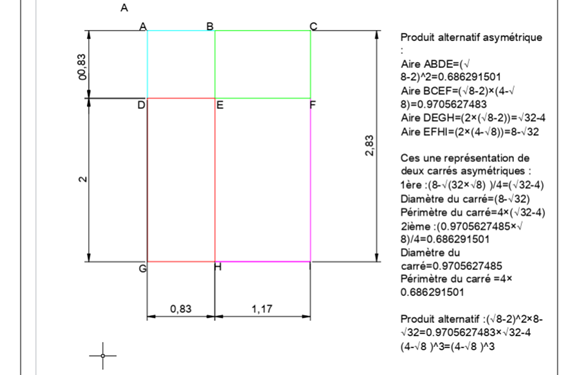
\includegraphics[width=0.85\textwidth]{asymetrique_alternatif_philippot.png}
    \caption{Analyse du mouvement de l'hypercube surface par surface -- Produit alternatif symétrique et asymétrique}
    \label{fig:hypercube}
\end{figure}

\subsection{Mouvement de l'hypercube surface par surface}

\subsubsection{Produit alternatif symétrique}

\begin{exemple}[: Calcul du produit alternatif symétrique]

\textbf{Carré A :}
\begin{itemize}
    \item Côté Carré A $= 1$
    \item Diamètre Carré A $= \sqrt{2}$
\end{itemize}

\textbf{Carré B :}
\begin{itemize}
    \item Côté Carré B $= 1.5$
    \item Diamètre Carré B $= \sqrt{4.5}$
\end{itemize}

\textbf{Produit alternatif à ajouter :}
\[
(1.5 \times 4) \times \sqrt{2} = \sqrt{4.5} \times 4
\]

\textbf{Résultat du produit :}
\[
\sqrt{72}
\]
\end{exemple}

\subsubsection{Produit alternatif asymétrique}

\begin{exemple}[: Calcul des aires -- Corrigé]
Les aires des différentes surfaces sont calculées comme suit :

\begin{align}
\text{Aire A} &= (\sqrt{8} - 2)^2 = 0.686291501 \\
\text{Aire B} &= 2 \times (4 - \sqrt{8}) \\
\text{Aire C} &= (\sqrt{8} - 2) \times (4 - \sqrt{8}) = 0.9705627485 \\
\text{Aire D} &= 2 \times (\sqrt{8} - 2) = \sqrt{32} - 4
\end{align}
\end{exemple}

\textbf{Transposition en relation périmètre-diamètre :}

Ce qui se transpose en :
\[
\text{Périmètre A} \times \text{Diamètre B} = \text{Diamètre A} \times \text{Périmètre B} \quad \text{(pour les aires)}
\]

\textbf{Produit alternatif corrigé :}
\[
0.9705627485 \times (\sqrt{32} - 4) = 0.686291501 \times 2 \times (4 - \sqrt{8})
\]

\textbf{Volume de l'hypercube :}
\[
(4 - \sqrt{8})^3 = (4 - \sqrt{8})^3 \quad \text{Volume de l'hypercube}
\]

\begin{resume}
Le résultat final pour le produit alternatif asymétrique révèle une valeur associable à un cube (puissance 3). Ce point permet d'associer le produit alternatif, à partir de surfaces de figures symétriques et asymétriques, au mouvement d'un tesseract en analysant son mouvement une surface à la fois.
\end{resume}

% ============================================================================
% SECTION 3 : ANALYSE NUMÉRIQUE MÉTRIQUE
% ============================================================================
\newpage
\section{Analyse Numérique Métrique}

Cette section présente une analyse numérique métrique en lien avec la fonction Zêta de Philippôt.

\begin{figure}[H]
    \centering
    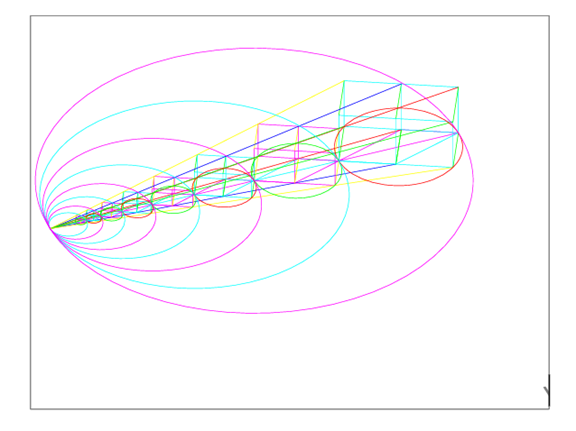
\includegraphics[width=0.9\textwidth]{analyse_numerique_metrique_cube.png}
    \caption{Représentation 3D de l'analyse numérique métrique -- Les cubes et pyramides internes}
    \label{fig:cube3d}
\end{figure}

\begin{resume}
L'analyse numerique metrique est une creation originale de l'auteur. Inspiree par un parallele avec l'analyse granulometrique, cette approche constitue le fondement de sa methode : une transposition conceptuelle ou la structure des tamis devient un outil pour comprendre la distribution des grandeurs numeriques.

Visuellement, l'auteur -- Philippe Thomas Savard -- represente cette idee par une serie de parallelogrammes successifs. Une droite centrale traverse chacun d'eux, tandis que deux autres droites, tangentes aux sommets formes par les angles obtus, encadrent la figure. Dans une analyse granulometrique classique, chaque tamis impose une limite de passant correspondant a une taille de maille precise. La masse retenue sur chaque tamis doit respecter une valeur determinee, et l'ensemble des resultats peut etre represente sous forme de courbe ou de zone ombree definissant les limites acceptables.

Dans l'analyse numerique metrique, cette zone ombree correspond a l'espace compris entre les deux droites tangentes aux sommets obtus des parallelogrammes. Ces sommets representent, en alternance, la position de la suite A et de la suite B. Comme nous le verrons plus loin, le nombre de termes dans ces deux suites determine la position du nombre premier associe au rapport spectral 1/2. Cette alternance est analogue au produit alternatif ou le perimetre du carre A multiplie par le diametre du carre B est egal au diametre du carre A multiplie par le perimetre du carre B.

Chaque parallelogramme possede deux sommets obtus, et chacun de ces sommets correspond successivement a la position de la suite A ou de la suite B. Cette alternance structure l'ensemble de la progression.

Lorsqu'une analyse granulometrique est effectuee sur un sol de calibre 0 mm a 20 mm, la serie de tamis utilisee est simple : tous les tamis sont inferieurs ou egaux a 20 mm. En revanche, pour un sol de calibre 0 mm a 56 mm, deux types de sols sont presents : un premier de 0 mm a 20 mm, et un second jusqu'a 56 mm. Dans ce cas, une substitution doit etre effectuee dans la serie de tamis afin d'eviter que l'operateur n'ait l'impression que les granulats "remontent" les tamis. Il faut donc remplacer un tamis de la serie 0--20 mm par celui de la serie 0--56 mm situe immediatement au-dessus.

L'auteur note egalement une analogie interessante observee dans le systeme de numeration grecque : la lettre zeta vaut 7 bien qu'elle occupe la sixieme position, en raison de l'ancienne presence du digamma entre l'epsilon et le zeta (reference : Encyclopedie libre Wikipedia, lettre grecque Zeta). Cette observation souleve une question similaire pour les nombres premiers, qui appartiennent a l'ensemble des entiers mais se distinguent des nombres composes. Deux types de nombres entrent donc en jeu.

Pour aborder l'enigme de Riemann, l'auteur imagine un monticule de cailloux plus haut que lui-meme, ou chaque caillou -- meme les poussieres -- porte un nombre, de 0 a l'infini. L'echantillon representatif utilise est constitue des dix chiffres 0 a 9, qui permettent de composer tous les nombres possibles. Lors du prelevement, la circonference et la hauteur du monticule sont mesurees. Grace a la normalisation des tamis et a l'espacement constant entre eux, il devient alors possible de retrouver la position exacte de chaque caillou dans le monticule.

L'analyse numerique metrique transpose cette logique : une serie de parallelogrammes se succedent, chacun defini par deux petites diagonales opposees. Ces diagonales entretiennent entre elles un rapport constant de 1/2, de l'interieur vers l'exterieur. En trois dimensions, cette structure devient une serie de paires de cubes, formant un volume analogue a un tesseract -- un hypercube en deformation continue.
\end{resume}

\subsection{Analyse numérique métrique mesure de la droite du haut.}

\begin{figure}[H]
    \centering
    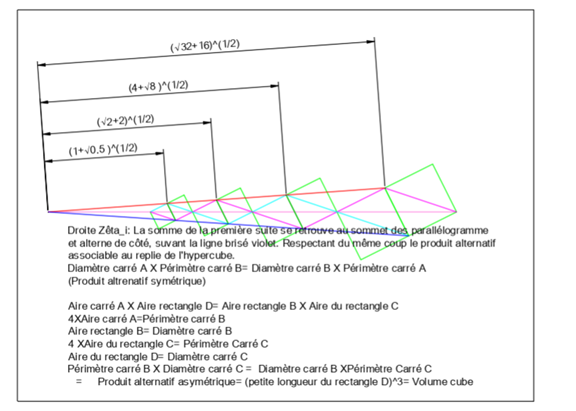
\includegraphics[width=0.85\textwidth]{analyse_numerique_metrique_haut.png}
    \caption{Vue de haut de l'analyse numérique métrique}
    \label{fig:anm_haut}
\end{figure}

\subsection{ Analyse numérique métrique, mesure de la droite du centre.}

\begin{figure}[H]
    \centering
    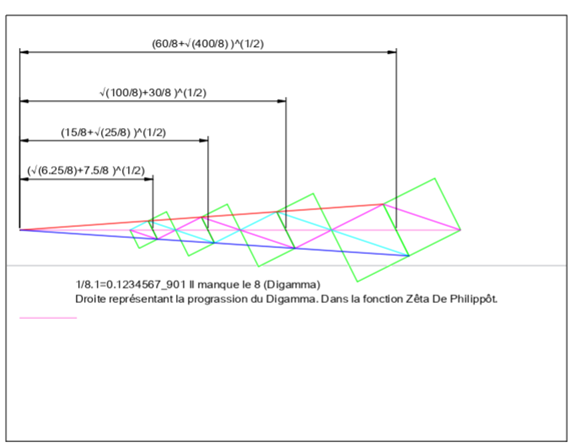
\includegraphics[width=0.85\textwidth]{analyse_numerique_metrique_centre.png}
    \caption{Analyse numérique métrique -- Vue centrale avec progression du Digamma}
    \label{fig:anm_centre}
\end{figure}

\begin{mydef}{Définition Zêta}
Dans le système de numération grecque, le Zêta vaut 7, bien qu'il occupe la sixième position. Ceci est dû à l'ancienne existence du Digamma, situé entre l'Epsilon et le Zêta.

\textit{(Définition tirée de l'encyclopédie libre Wikipédia)}

Cette particularité -- une valeur qui ne correspond pas à la position -- rejoint l'idée de substitution évoquée dans l'analyse granulométrique qui comme pour la méthode lié au sol permet le tamisage d'un sol composé de deux granulat permet du a la substitution dans la suite B de comparer les nombres composés et les nombres premiers.
\end{mydef}

\subsection{Géométrie des suites. Aires des trapèzes.}

\begin{figure}[H]
    \centering
    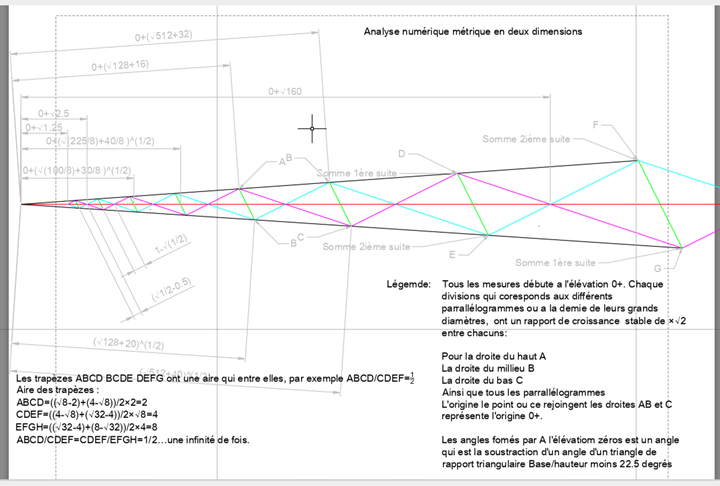
\includegraphics[width=0.9\textwidth]{analyse_numerique_metrique_aire_trapeze.png}
    \caption{Analyse numérique métrique en deux dimensions -- Aires des trapèzes}
    \label{fig:trapeze}
\end{figure}

Les deux suites (la première A et la deuxième B) utilisées pour déterminer la valeur des nombres premiers sont définies par les parallélogrammes qui constitue l'analyse numérique métrique à l'intérieur des rectangles. Ces parallélogrammes sont traversés le long de la grande diagonal, passant par leurs centres longitudinaux.

\begin{exemple}[: Calcul des aires des trapèzes]
Les lettres A, B, C, D, E, F, G, H forment trois trapèzes successifs : ABCD, CDEF et EFGH. Les aires de ces trapèzes présentent une propriété remarquable : une fois mises en relation, elles entretiennent entre elles un rapport constant de $\frac{1}{2}$.

\textbf{Calculs :}
\begin{align}
\text{Aire ABCD} &= \frac{(\sqrt{2}-1) + (2-\sqrt{2})}{2} \times 1 = 0.5 \\
\text{Aire CDEF} &= \frac{(2-\sqrt{2}) + (\sqrt{8}-2)}{2} \times \sqrt{2} = 1 \\
\text{Aire EFGH} &= \frac{(\sqrt{8}-2) + (4-\sqrt{8})}{2} \times 2 = 2
\end{align}

\textbf{Mise en relation des aires :}
\[
\frac{0.5}{1} = \frac{1}{2} \quad \text{et} \quad \frac{1}{2} = \frac{1}{2}
\]
\end{exemple}

\begin{resume}
À cette étape, les aires des trapèzes une évidence intuitive -- que les parties réelles des zéros non triviaux de la fonction zêta pourraient toutes être égales à $\frac{1}{2}$.
\end{resume}

% ============================================================================
% SECTION 4 : MÉTHODE DE PHILIPPÔT - VALIDATION HOL COMPLÈTE
% ============================================================================
\newpage
\section{La Méthode de Philippôt -- Validation Isabelle/HOL}

La méthode de Philippôt constitue la première étape dans un effort visant à déterminer les nombres premiers. Il s'agit d'une approche itérative, fondée sur des suites fractionnaires, dont la somme produit un résultat fini à chaque étape.

\begin{resume}
\textbf{Imaginez} une série de fractions comme les marches d'un escalier : chaque marche est exactement la moitié de la précédente. En montant cet escalier, vous vous rapprochez toujours plus d'un plafond (la valeur 1), sans jamais l'atteindre complètement, sauf si vous suivez les règles précises de la méthode.
\end{resume}

\subsection{Script HOL Complet : methode\_de\_philippot.thy}

\begin{holcode}[title={\textcolor{white}{Fichier : methode\_de\_philippot.thy -- COMPLET}}]
\begin{lstlisting}
theory methode_de_philippot
  imports Main "HOL.Rat"
begin

section "Géométrie du spectre premier – methode de Philippot."

text "
  Ce fichier contient les définitions, structures et mécanismes nécessaires
  à l'étude de la géométrie du spectre premier, incluant la méthode de Philippôt.
"

subsection "Étape 1 : suites explicites pour 3 à 11 termes"

definition etape1_3 :: "rat list" where
  "etape1_3 = [1/2, 1/3, 1/6]"

definition etape1_4 :: "rat list" where
  "etape1_4 = [1/2, 1/4, 1/6, 1/12]"

definition etape1_5 :: "rat list" where
  "etape1_5 = [1/2, 1/4, 1/8, 1/12, 1/24]"

definition etape1_6 :: "rat list" where
  "etape1_6 = [1/2, 1/4, 1/8, 1/16, 1/24, 1/48]"

definition etape1_7 :: "rat list" where
  "etape1_7 = [1/2, 1/4, 1/8, 1/16, 1/32, 1/48, 1/96]"

definition etape1_8 :: "rat list" where
  "etape1_8 = [1/2, 1/4, 1/8, 1/16, 1/32, 1/64, 1/96, 1/192]"

definition etape1_9 :: "rat list" where
  "etape1_9 = [1/2, 1/4, 1/8, 1/16, 1/32, 1/64, 1/128, 1/192, 1/384]"

definition etape1_10 :: "rat list" where
  "etape1_10 = [1/2, 1/4, 1/8, 1/16, 1/32, 1/64, 1/128, 1/256, 1/384, 1/768]"

definition etape1_11 :: "rat list" where
  "etape1_11 = [1/2, 1/4, 1/8, 1/16, 1/32, 1/64, 1/128, 1/256, 1/512, 1/768, 1/1536]"


subsection "Structure réglementaire des suites à l'étape 1"

fun etape1_general :: "nat ⇒ rat list" where
  "etape1_general n =
     (if n < 3 then []
      else
        let
          base = map (λi. 1 / (2 ^ i)) [1 ..< n - 1];
          avant = (1 / (2 ^ (n - 2))) * (2/3);
          dernier = avant / 2
        in base @ [avant, dernier])"

definition suite_reglementaire_etape1 :: "nat ⇒ rat list ⇒ bool" where
  "suite_reglementaire_etape1 n xs ⟷
     length xs = n ∧
     n ≥ 3 ∧
     (∀i. 1 ≤ i ∧ i ≤ n - 2 ⟶ xs ! (i - 1) = 1 / (2 ^ i)) ∧
     xs ! (n - 2) = xs ! (n - 3) * (2/3) ∧
     xs ! (n - 1) = xs ! (n - 2) / 2"


subsection "Règle générale de substitution (toutes étapes ≥ 2)"

text "
  La position de substitution dépend uniquement du nombre de termes n :
  – pour 3 ≤ n ≤ 7, la position de substitution est n - 2 (1, 2, 3, 4, 5) ;
  – pour n ≥ 8, la position de substitution est fixée à 6.
"

definition pos_substitution :: "nat ⇒ nat" where
  "pos_substitution n =
     (if n < 3 then 0
      else if n ≤ 7 then n - 2
      else 6)"


subsection "Étape 2 : suites explicites pour 3 à 7 termes"

definition etape2_3 :: "rat list" where
  "etape2_3 = [1/4, 1/6, 1/12]"

definition etape2_4 :: "rat list" where
  "etape2_4 = [1/2, 1/8, 1/12, 1/24]"

definition etape2_5 :: "rat list" where
  "etape2_5 = [1/2, 1/4, 1/16, 1/24, 1/48]"

definition etape2_6 :: "rat list" where
  "etape2_6 = [1/2, 1/4, 1/8, 1/32, 1/48, 1/96]"

definition etape2_7 :: "rat list" where
  "etape2_7 = [1/2, 1/4, 1/8, 1/16, 1/64, 1/96, 1/192]"

definition suite_reglementaire_etape2_petit ::
  "nat ⇒ rat list ⇒ bool" where
  "suite_reglementaire_etape2_petit n xs ⟷
     length xs = n ∧ 3 ≤ n ∧ n ≤ 7 ∧
     xs ! (n - 2) = xs ! (n - 3) * (2/3) ∧
     sum_list xs = 1 - xs ! (pos_substitution n - 1)"

definition suite_reglementaire_etape2_grand ::
  "nat ⇒ rat list ⇒ bool" where
  "suite_reglementaire_etape2_grand n xs ⟷
     length xs = n ∧ n ≥ 8 ∧
     xs ! (n - 2) = xs ! (n - 3) * (2/3) ∧
     pos_substitution n = 6 ∧
     sum_list xs = 1 - (1/64)"


subsection "Étape 3 : suites explicites pour 7 termes et moins"

text "
  L'étape 3 répète le mécanisme de l'étape 2 :
  une position est substituée, et une valeur compensatoire est ajoutée
  de l'autre côté de l'égalité. La position de substitution est la même
  que pour l'étape 2 pour un nombre de termes donné.
"

definition etape3_3 :: "rat list" where
  "etape3_3 = [1/24, 1/12, 1/8]"

definition etape3_4 :: "rat list" where
  "etape3_4 = [1/48, 1/24, 1/16, 1/2]"

definition etape3_5 :: "rat list" where
  "etape3_5 = [1/96, 1/48, 1/32, 1/4, 1/2]"

definition etape3_6 :: "rat list" where
  "etape3_6 = [1/192, 1/96, 1/64, 1/8, 1/4, 1/2]"

definition etape3_7 :: "rat list" where
  "etape3_7 = [1/192, 1/96, 1/128, 1/16, 1/8, 1/4, 1/2]"

definition valeur_substituee_etape3 :: "nat ⇒ rat" where
  "valeur_substituee_etape3 n =
     (if n = 3 then 1/2 + 1/4
      else if n = 4 then 1/4 + 1/8
      else if n = 5 then 1/8 + 1/16
      else if n = 6 then 1/16 + 1/32
      else if n = 7 then 1/32 + 1/64
      else 0)"

definition suite_reglementaire_etape3 ::
  "nat ⇒ rat list ⇒ bool" where
  "suite_reglementaire_etape3 n xs ⟷
     length xs = n ∧ 3 ≤ n ∧ n ≤ 7 ∧
     sum_list xs = 1 - valeur_substituee_etape3 n"


subsection "Étape 3 : suites explicites pour 8 termes et plus"

definition etape3_8 :: "rat list" where
  "etape3_8 =
     [1/384, 1/192, 1/128, 1/32, 1/16, 1/8, 1/4, 1/2]"

definition etape3_9 :: "rat list" where
  "etape3_9 =
     [1/768, 1/384, 1/256, 1/128, 1/32, 1/16, 1/8, 1/4, 1/2]"

definition etape3_10 :: "rat list" where
  "etape3_10 =
     [1/1536, 1/768, 1/512, 1/256, 1/128, 1/32, 1/16, 1/8, 1/4, 1/2]"

definition etape3_11 :: "rat list" where
  "etape3_11 =
     [1/3072, 1/1536, 1/1024, 1/512, 1/256, 1/128, 1/32, 1/16, 1/8, 1/4, 1/2]"

definition valeur_substituee_etape3_grand :: "rat" where
  "valeur_substituee_etape3_grand = (1/64 + 1/128)"

definition suite_reglementaire_etape3_grand ::
  "nat ⇒ rat list ⇒ bool" where
  "suite_reglementaire_etape3_grand n xs ⟷
     length xs = n ∧ n ≥ 8 ∧
     pos_substitution n = 6 ∧
     sum_list xs = 1 - valeur_substituee_etape3_grand"


subsection "Propriété fondamentale des puissances de deux"

lemma ratio_puissances_de_deux:
  fixes n :: nat
  shows "(1 / (2 ^ (Suc n)) :: rat) / (1 / (2 ^ n)) = 1 / 2"
  by (simp add: field_simps)

lemma exemples_ratio_puissances_de_deux:
  shows "(1/128 :: rat) / (1/64) = 1/2"
    and "(1/64 :: rat) / (1/32) = 1/2"
    and "(1/32 :: rat) / (1/16) = 1/2"
    and "(1/16 :: rat) / (1/8) = 1/2"
    and "(1/8 :: rat) / (1/4) = 1/2"
    and "(1/4 :: rat) / (1/2) = 1/2"
  by (simp_all add: ratio_puissances_de_deux)

subsection "Structure spectrale generale pour n termes et infinite d'etapes"

text "
  Dans cette section, on formalise la structure purement spectrale des puissances de deux,
  independante des substitutions specifiques des etapes 1, 2 et 3.

  Idee centrale :
  – chaque terme est de la forme 1 / 2^i (i ≥ 1) ;
  – le rapport entre deux termes consecutifs est toujours 1/2 ;
  – cette propriete vaut pour toute longueur finie n, et conceptuellement pour une infinite de termes.
"

definition terme_spectral :: "nat ⇒ rat" where
  "terme_spectral i = 1 / (2 ^ i)"

definition suite_spectrale :: "nat ⇒ rat list" where
  "suite_spectrale n = map terme_spectral [1 ..< Suc n]"

text "
  Propriete spectrale locale : pour tout i ≥ 1,
  le rapport entre le terme i+1 et le terme i est exactement 1/2.
"

lemma ratio_spectral_local:
  fixes i :: nat
  assumes "i ≥ 1"
  shows "terme_spectral (Suc i) / terme_spectral i = (1/2 :: rat)"
proof -
  have "terme_spectral (Suc i) / terme_spectral i
        = (1 / (2 ^ (Suc i))) / (1 / (2 ^ i))"
    by (simp add: terme_spectral_def)
  also have "... = (1/2 :: rat)"
    using ratio_puissances_de_deux[of i] by simp
  finally show ?thesis .
qed

text "
  Interpretation :
  – la definition "terme_spectral" encode une infinite de termes 1 / 2^i, i ≥ 1 ;
  – le lemme "ratio_spectral_local" montre que le rapport entre deux termes consecutifs
    est toujours 1/2, pour tout i ;
  – en prolongeant i sans borne, on obtient une structure spectrale qui produit 1/2
    une infinite de fois, de manière purement arithmetique.
"

end

\end{lstlisting}
\end{holcode}

\subsection{Tableau fractionnaire -- Etape 1}

\begin{center}
\scriptsize
\begin{tabular}{|c|c|c|c|c|c|c|c|c|c|c|c|c|}
\hline
\textbf{Pos.} & 11 & 10 & 9 & 8 & 7 & 6 & 5 & 4 & 3 & 2 & 1 & \textbf{Somme} \\
\hline
& & & & & & & & $\frac{1}{6}$ & $\frac{1}{3}$ & $\frac{1}{2}$ & & = 1 \\
\hline
& & & & & & & $\frac{1}{12}$ & $\frac{1}{6}$ & $\frac{1}{4}$ & $\frac{1}{2}$ & & = 1 \\
\hline
& & & & & & $\frac{1}{24}$ & $\frac{1}{12}$ & $\frac{1}{8}$ & $\frac{1}{4}$ & $\frac{1}{2}$ & & = 1 \\
\hline
& & & & & $\frac{1}{48}$ & $\frac{1}{24}$ & $\frac{1}{16}$ & $\frac{1}{8}$ & $\frac{1}{4}$ & $\frac{1}{2}$ & & = 1 \\
\hline
& & & & $\frac{1}{96}$ & $\frac{1}{48}$ & $\frac{1}{32}$ & $\frac{1}{16}$ & $\frac{1}{8}$ & $\frac{1}{4}$ & $\frac{1}{2}$ & & = 1 \\
\hline
& & & $\frac{1}{192}$ & $\frac{1}{96}$ & $\frac{1}{64}$ & $\frac{1}{32}$ & $\frac{1}{16}$ & $\frac{1}{8}$ & $\frac{1}{4}$ & $\frac{1}{2}$ & & = 1 \\
\hline
& & $\frac{1}{384}$ & $\frac{1}{192}$ & $\frac{1}{128}$ & $\frac{1}{64}$ & $\frac{1}{32}$ & $\frac{1}{16}$ & $\frac{1}{8}$ & $\frac{1}{4}$ & $\frac{1}{2}$ & & = 1 \\
\hline
& $\frac{1}{768}$ & $\frac{1}{384}$ & $\frac{1}{256}$ & $\frac{1}{128}$ & $\frac{1}{64}$ & $\frac{1}{32}$ & $\frac{1}{16}$ & $\frac{1}{8}$ & $\frac{1}{4}$ & $\frac{1}{2}$ & & = 1 \\
\hline
$\frac{1}{1536}$ & $\frac{1}{768}$ & $\frac{1}{512}$ & $\frac{1}{256}$ & $\frac{1}{128}$ & $\frac{1}{64}$ & $\frac{1}{32}$ & $\frac{1}{16}$ & $\frac{1}{8}$ & $\frac{1}{4}$ & $\frac{1}{2}$ & & = 1 \\
\hline
\end{tabular}
\end{center}

\begin{resume}
\textbf{Interpretation :} Ce resultat montre que le rapport entre deux puissances successives de $\frac{1}{2}$ est toujours constant et égal à $\frac{1}{2}$. Comme une chaîne où chaque maillon est exactement la moitié du précédent, cette propriété reste vraie jusqu'à l'infini.
\end{resume}

% ============================================================================
% TABLEAUX METHODE DE PHILIPPÔT - =ETAPES 2 ET 3 (CORRECTION AJOUTEE)
% ============================================================================

\subsection{Methode de Philippot -- Tableau des Etapes 2 et 3}
\begin{center}
\scriptsize
\begin{tabular}{|c|c|c|c|c|c|c|c|c|c|c|c|c|}
\hline
11 & 10 & 9 & 8 & 7 & 6 & 5 & 4 & 3 & 2 & 1 & Pos. & Som. \\
\hline
 &  &  &  &  &  &  &  & 1/12 & + 1/6 & + 1/4 &  & = 1 - 1/2 \\
\hline
 &  &  &  &  &  &  & 1/24 & + 1/12 & + 1/8 & + 1/2 &  & = 1 - 1/4 \\
\hline
 &  &  &  &  &  & 1/48 & + 1/24 & + 1/16 & + 1/4 & + 1/2 &  & = 1 - 1/8 \\
\hline
 &  &  &  &  & 1/96 & + 1/48 & + 1/32 & + 1/8 & + 1/4 & + 1/2 &  & = 1 - 1/16 \\
\hline
 &  &  &  & 1/192 & + 1/96 & + 1/64 & + 1/16 & + 1/8 & + 1/4 & + 1/2 &  & = 1 - 1/32 \\
\hline
\end{tabular}
\end{center}

\vspace{0.5cm}

\begin{center}
\textbf{Tableau Etape 3 -- Methode de Philippôt}
\end{center}

\begin{center}
\scriptsize
\begin{tabular}{|c|c|c|c|c|c|c|c|c|c|c|c|c|}
\hline
11 & 10 & 9 & 8 & 7 & 6 & 5 & 4 & 3 & 2 & 1 & \textbf{Positions} & \textbf{Sommes} \\
\hline
 &  &  &  &  &  &  &  & $\frac{1}{24}$ & $\frac{1}{12}$ & $\frac{1}{8}$ & 2\;1 & $= 1 - \left(\frac{1}{2} + \frac{1}{4}\right)$ \\
\hline
 &  &  &  &  &  &  & $\frac{1}{48}$ & $\frac{1}{24}$ & $\frac{1}{16}$ & $\frac{1}{2}$ & 3\;1 & $= 1 - \left(\frac{1}{4} + \frac{1}{8}\right)$ \\
\hline
 &  &  &  &  &  & $\frac{1}{96}$ & $\frac{1}{48}$ & $\frac{1}{32}$ & $\frac{1}{4}$ & $\frac{1}{2}$ & 4\;1 & $= 1 - \left(\frac{1}{8} + \frac{1}{16}\right)$ \\
\hline
 &  &  &  &  & $\frac{1}{192}$ & $\frac{1}{96}$ & $\frac{1}{64}$ & $\frac{1}{8}$ & $\frac{1}{4}$ & $\frac{1}{2}$ & 5\;1 & $= 1 - \left(\frac{1}{16} + \frac{1}{32}\right)$ \\
\hline
 &  &  &  & $\frac{1}{192}$ & $\frac{1}{96}$ & $\frac{1}{128}$ & $\frac{1}{16}$ & $\frac{1}{8}$ & $\frac{1}{4}$ & $\frac{1}{2}$ & 6\;1 & $= 1 - \left(\frac{1}{32} + \frac{1}{64}\right)$ \\
\hline
\end{tabular}
\end{center}

\begin{resume}
\textbf{Interpretation des Etapes 2 et 3 :} Ces tableaux illustrent la progression de la méthode de Philippôt où une position est substituée à chaque étape. La valeur substituée est multipliée par $\frac{1}{2}$ par rapport à l'étape précédente, créant ainsi une structure fractionnaire cohérente qui converge vers les propriétés des nombres premiers.
\end{resume}

\begin{center}
\textbf{Tableau Etape 3 pour 8 termes et plus -- Methode de Philippôt}
\end{center}

\begin{center}
\scriptsize
\begin{tabular}{|c|c|c|c|c|c|c|c|c|c|c|c|c|}
\hline
11 & 10 & 9 & 8 & 7 & 6 & 5 & 4 & 3 & 2 & 1 & \textbf{Positions} & \textbf{Sommes} \\
\hline
 &  &  & $\frac{1}{768}$ & $\frac{1}{384}$ & $\frac{1}{256}$ & $\frac{1}{32}$ & $\frac{1}{16}$ & $\frac{1}{8}$ & $\frac{1}{4}$ & $\frac{1}{2}$ &  & $= 1 - \left(\frac{1}{64} + \frac{1}{128}\right)$ \\
\hline
 &  & $\frac{1}{1536}$ & $\frac{1}{768}$ & $\frac{1}{512}$ & $\frac{1}{256}$ & $\frac{1}{32}$ & $\frac{1}{16}$ & $\frac{1}{8}$ & $\frac{1}{4}$ & $\frac{1}{2}$ &  & $= 1 - \left(\frac{1}{64} + \frac{1}{128}\right)$ \\
\hline
 & $\frac{1}{3072}$ & $\frac{1}{1536}$ & $\frac{1}{1024}$ & $\frac{1}{512}$ & $\frac{1}{256}$ & $\frac{1}{32}$ & $\frac{1}{16}$ & $\frac{1}{8}$ & $\frac{1}{4}$ & $\frac{1}{2}$ &  & $= 1 - \left(\frac{1}{64} + \frac{1}{128}\right)$ \\
\hline
$\frac{1}{6144}$ & $\frac{1}{3072}$ & $\frac{1}{2048}$ & $\frac{1}{1024}$ & $\frac{1}{512}$ & $\frac{1}{256}$ & $\frac{1}{32}$ & $\frac{1}{16}$ & $\frac{1}{8}$ & $\frac{1}{4}$ & $\frac{1}{2}$ &  & $= 1 - \left(\frac{1}{64} + \frac{1}{128}\right)$ \\
\hline
\end{tabular}
\end{center}

% ============================================================================
% SECTION 4.3 : RAPPORT SPECTRAL GENERALISE
% ============================================================================

\[
\textbf{Rapport spectral generalise :}\qquad
\frac{\displaystyle \frac{1}{2^{\,n+1}}}{\displaystyle \frac{1}{2^{\,n}}}
\;=\;
\frac{1}{2}
\qquad\text{pour tout } n \ge 0.
\]

\[
\textbf{Forme iterative :}\qquad
\frac{1/256}{1/128}
=
\frac{1/128}{1/64}
=
\frac{1/64}{1/32}
=
\cdots
=
\frac{1}{2},
\quad
\text{repete a l'infini.}
\]

\[
\textbf{Forme entierement generalisee :}\qquad
\frac{\displaystyle \frac{1}{n_1}}{\displaystyle \frac{1}{n_2}}
=
\frac{n_2}{n_1}
=
\frac{1}{2}
\quad\text{des que}\quad
n_2 = 2n_1.
\]

\textbf{Resume explicatif (FR).} \\
Cette equation exprime la propriete fondamentale des puissances de deux : chaque terme
est exactement la moitie du precedent. Ainsi, le rapport entre deux inverses consecutifs
de puissances de deux est toujours egal a 1/2. Cette relation est stable, repetitive
et se propage indefiniment lorsque l'on itere la structure. Elle constitue le noyau
spectral de la methode, garantissant une coherence interne parfaite entre les niveaux
successifs.

% ============================================================================
% SECTION 5 : NOMBRES PREMIERS ET DIGAMMA
% ============================================================================
\newpage
\section{Les Nombres Premiers et l'Emploi du Digamma}

Determiner les nombres premiers est une autre methode iterative, mais cette fois deux suites sont necessaires. Deux suites de racines carrees forment un rapport triangulaire base/hauteur = 1/2.

\begin{mydef}{Suites pour les nombres premiers}
Pour le nombre premier (29), qui est le 10\textsuperscript{e} nombre premier, deux suites de 10 racines carrees, qui sont le produit de la proposition $\sqrt{a^2 + b^2}$, forment les deux suites. Les deux suites ont toujours la meme quantite de termes lorsqu'il s'agit du meme nombre premier.
\end{mydef}

\subsection{Exemple : Determiner le nombre premier (5)}

Commencons par 3 termes, le 3\textsuperscript{e} nombre premier etant (5).

La suite fractionnaire egale a 1 pour trois fractions :
\[
\frac{1}{6} + \frac{1}{3} + \frac{1}{2} = 1
\]

\begin{exemple}[: Calcul de la premiere suite pour (5)]
\textbf{Premier terme :}
\[
\left(\frac{\sqrt{1.25}}{2} - \frac{1}{2}\right) \times 4 + 2 = \sqrt{5}
\]
Ou $(1^2 + 2^2)^{1/2} = \sqrt{5}$

\textbf{Deuxieme terme :}
\[
\left(\frac{\sqrt{1.25}}{2} - \frac{1}{3}\right) \times 6 + 2 = \sqrt{11.25}
\]
Ou $(1.5^2 + 3^2)^{1/2} = \sqrt{11.25}$

\textbf{Troisieme terme :}
\[
\left(\frac{\sqrt{1.25}}{2} - \frac{1}{6}\right) \times 12 + 2 = \sqrt{45}
\]
Ou $(3^2 + 6^2)^{1/2} = \sqrt{45}$

\textbf{Somme de la premiere suite de (5) :}
\[
\sqrt{45} + \sqrt{11.25} + \sqrt{5} = \sqrt{151.25}
\]

\textbf{Equation de verification finale :}
\[
\left( \frac{\sqrt{13.203125}}{2} \times 2^{3} \right) - \sqrt{5}
= \sqrt{151.25}.
\]
\end{exemple}

\subsection{Tableau des valeurs de l'intervalle 29, 31, 37, 41}

\begin{center}
\begin{tabular}{|c|c|c|}
\hline
\textbf{Nombre premier} & \textbf{Calcul Digamma} & \textbf{Valeur Digamma} \\
\hline
29 & $-\sqrt{81920}$ & $= -\sqrt{81920}$ \\
\hline
31 & $+5\sqrt{81920}$ & $= \sqrt{204800}$ \\
\hline
37 & $+9\sqrt{81920} + 5\sqrt{184320}$ & $= \sqrt{22302720}$ \\
\hline
41 & $+13\sqrt{81920} + 9\sqrt{184320} + 5\sqrt{737280}$ & $= \sqrt{141086720}$ \\
\hline
\end{tabular}
\end{center}

% ============================================================================
% CORRECTION 5.2 : EXEMPLES ET TABLEAU POUR LE NOMBRE PREMIER 31
% ============================================================================
\subsection{Exemple complet : Determiner le nombre premier (31)}

Le nombre premier 31 est le 11\textsuperscript{ieme} nombre premier. Voici le tableau de la somme des deux suites pour 11 termes :

\begin{center}
\textbf{Tableau de la somme de la 1\textsuperscript{ere} et 2\textsuperscript{ieme} suite (31), 11\textsuperscript{ieme} nombre premier}
\end{center}

\begin{center}
\small
\begin{tabular}{|c|c|c|}
\hline
\textbf{Position} & \textbf{1\textsuperscript{ere} suite} & \textbf{2\textsuperscript{ieme} suite} \\
\hline
1 & $\sqrt{5}$ & $\sqrt{5}$ \\
\hline
2 & $\sqrt{20}$ & $\sqrt{20}$ \\
\hline
3 & $\sqrt{80}$ & $\sqrt{80}$ \\
\hline
4 & $\sqrt{320}$ & $\sqrt{320}$ \\
\hline
5 & $\sqrt{1280}$ & $\sqrt{1280}$ \\
\hline
6 & $\sqrt{5120}$ & $\sqrt{5120}$ \\
\hline
7 & $\sqrt{20480}$ & $\sqrt{20480}$ \\
\hline
8 & $\sqrt{81920}$ & $\sqrt{81920}$ \\
\hline
9 & $\sqrt{327680}$ & $\sqrt{327680}$ \\
\hline
10 & $\sqrt{983040}$ & $\sqrt{1966080}$ \\
\hline
11 & $\sqrt{3932160}$ & $\sqrt{7864320}$ \\
\hline
\end{tabular}
\end{center}

\subsubsection{Verification}

\textbf{Somme de la 1\textsuperscript{ere} suite :}
\[
\sqrt{5} + \sqrt{20} + \sqrt{80} + \sqrt{320} + \sqrt{1280} + \sqrt{5120} + \sqrt{20480} + \sqrt{81920} + \sqrt{327680} + \sqrt{983040} + \sqrt{3932160}
\]
\[
= \sqrt{13827845}
\]

\textbf{Somme de la 2\textsuperscript{ieme} suite :}
\[
\sqrt{5} + \sqrt{20} + \sqrt{80} + \sqrt{320} + \sqrt{1280} + \sqrt{5120} + \sqrt{20480} + \sqrt{81920} + \sqrt{327680} + \sqrt{1966080} + \sqrt{7864320}
\]
\[
= \sqrt{54285125}
\]

\textbf{Digamma :} $+5\sqrt{81920}$

\textbf{Digamma calcule :}
\[
\text{Somme 1\textsuperscript{ere} suite} + \text{Digamma} = \text{Digamma calcule}
\]
\[
\sqrt{13827845} + 5\sqrt{81920} = \sqrt{26519045}
\]

\textbf{Determination du nombre premier 31 :}
\[
\frac{\sqrt{54285125} - \sqrt{26519045}}{\sqrt{5120}} = 31
\]

\subsubsection{Verification alternative}
\[
(\sqrt{54285125} - 31) \times \sqrt{5120} = \sqrt{26519045} \quad \text{(Digamma calcule)}
\]

\section*{Methodes Spectrales : Exemples pour le rapport 1/2}

\subsection*{Exemple pour le nombre premier 31 (11ieme nombre premier, 11 termes)}

2+4+8+16+32+64+128+256+512+768+1536 = 3326 Somme suite A(31).\\
2+4+8+16+32+128+256+512+1024+1536+3072 = 6590 Somme suite B(31).\\

\[
\left(\frac{3.25}{2} \cdot 2^{11}\right) - 2 = 3326 \quad \text{somme suite A.}
\]

\[
\left(\frac{6.5}{2} \cdot 2^{11}\right) - 66 = 6590 \quad \text{somme suite B.}
\]

Digamma : \(5 \cdot 256 = 1280\).\\
Digamma calcule : \(3326 + 1280 = 4606\).\\

\[
\frac{6590 - 4606}{64} = 31 \quad \text{11ieme nombre premier.}
\]

\bigskip

\subsection*{Exemple pour le nombre premier 29 (10ieme nombre premier, 10 termes)}

2+4+8+16+32+64+128+256+384+768 = 1662 Somme suite A(29).\\
2+4+8+16+32+128+256+512+768+1536 = 3262 Somme suite B(29).\\

\[
\left(\frac{3.25}{2} \cdot 2^{10}\right) - 2 = 1662
\]

\[
\left(\frac{6.5}{2} \cdot 2^{10}\right) - 66 = 3262
\]

Digamma (8ieme position) : \(256\).\\
Digamma calcule : \(1662 - 256 = 1406\).\\

\[
(3262/64 - 29) \cdot 64 = 1406
\]

\[
\frac{3262 - 1406}{64} = 29 \quad \text{10ieme nombre premier.}
\]

\bigskip

\subsection*{Exemple pour le nombre premier 23 (9ieme nombre premier)}

2+3+4+8+16+32+64+128+192+384 = 830 Somme 1ere suite (23).\\
2+4+8+16+32+128+256+384+768 = 1598 Somme 2ieme suite (23).\\

Digamma calcule :

\[
(1598/64 - 23) \cdot 64 = 126
\]

\[
\frac{1598 - 126}{64} = 23 \quad \text{9ieme nombre premier.}
\]

\[
\left(\frac{3.25}{2} \cdot 2^{n}\right) - 2 = \text{somme 1ere suite.}
\]

\[
\left(\frac{6.5}{2} \cdot 2^{n}\right) - 66 = \text{somme 2ieme suite.}
\]

Quand \(n\) est un entier strictement positif, \(n\) correspond a la position du nombre premier et a la quantite de termes dans la suite.\\
Lorsque 2 = 1er, 3 = 2e, 5 = 3e, ... alors \(P_{n} = n\)-ieme.

\bigskip

\subsection*{Exemple pour le nombre premier 37 (12ieme nombre premier, 12 termes)}

2+4+8+16+32+64+128+256+512+1024+1536+3072 = 6654 Somme suite A.\\
2+4+8+16+32+128+256+512+1024+2048+3072+6144 = 13246 Somme suite B.\\

\[
\left(\frac{3.25}{2} \cdot 2^{12}\right) - 2 = 6654
\]

\[
\left(\frac{6.5}{2} \cdot 2^{12}\right) - 66 = 13246
\]

Digamma(37) : \(9 \cdot 256 + 5 \cdot 384 = 4224\).\\
Digamma calcule : \(6654 + 4224 = 10878\).\\

\[
\frac{13246 - 10878}{64} = 37 \quad \text{12ieme nombre premier.}
\]

\bigskip

\subsection*{Exemple pour le nombre premier 41 (13ieme nombre premier, 13 termes)}

2+4+8+16+32+64+128+256+512+1024+2048+3072+6144 = 13310 Somme suite A.\\
2+4+8+16+32+128+256+512+1024+2048+4096+6144+12288 = 26558 Somme suite B.\\

\[
\left(\frac{3.25}{2} \cdot 2^{13}\right) - 2 = 13310
\]

\[
\left(\frac{6.5}{2} \cdot 2^{13}\right) - 66 = 26558
\]

Digamma(41) : \(13 \cdot 256 + 9 \cdot 384 + 5 \cdot 768 = 10624\).\\
Digamma calcule : \(13310 + 10624 = 23934\).\\

\[
\frac{26558 - 23934}{64} = 41 \quad \text{13ieme nombre premier.}
\]

\bigskip

\subsection*{Distance spectrale (comparaison 1 a 1)}

Comparaison de nombres premiers 1*1 :

\[
\frac{
\left(\frac{3.25}{2} \cdot 2^{n_{1}} - 2\right)
-
\left(\frac{3.25}{2} \cdot 2^{n_{2}} - 2\right)
}{
\left(\frac{6.5}{2} \cdot 2^{n_{1}} - 66\right)
-
\left(\frac{6.5}{2} \cdot 2^{n_{2}} - 66\right)
}
= \frac{1}{2}
\]

Toujours.

\[
\text{Ordonnee :}\qquad
R_{\mathrm{ord}}(A,B)
=
\frac{\displaystyle \sum_{n \in A} A(n)\;-\;\sum_{n \in B} A(n)}
     {\displaystyle \sum_{n \in A} B(n)\;-\;\sum_{n \in B} B(n)}
\qquad\text{avec}\quad |B| = |A| + 1,\; \max(A) < \min(B),
\]
\[
R_{\mathrm{ord}}(A,B) \;\neq\; \frac{1}{2}.
\]

\textbf{Resume explicatif (Ordonnee).} \\
Dans le cas ordonne, les blocs A et B respectent une structure strictement croissante
et decalee d'une unite. Malgre cette organisation rigoureuse, le rapport obtenu n'est
pas egal à $1/2$. Cela montre que l'alignement des puissances et la progression
structurelle ne suffisent pas à produire la symetrie spectrale attendue. Le systeme
ordonne reste coherent, mais il ne conduit pas au rapport $1/2$.

\[
\text{Chaotique :}\qquad
R_{\mathrm{chaos}}(A,B)
=
\frac{\displaystyle \sum_{n \in A} A(n)\;-\;\sum_{n \in B} A(n)}
     {\displaystyle \sum_{n \in A} B(n)\;-\;\sum_{n \in B} B(n)}
\qquad\text{avec}\quad |A| \neq |B|,\; \neg\,\text{Ordonnée}(A,B),
\]
\[
R_{\mathrm{chaos}}(A,B) \;=\; 0.5 \;+\; \text{faible reste}.
\]

\textbf{Resume explicatif (Chaotique).} \\
Dans le cas chaotique, les blocs A et B ne respectent plus la structure ordonnee :
leurs longueurs diffèrent et leurs puissances ne sont plus alignees. Cette absence
d'organisation cree une compensation arithmetique qui rapproche le rapport de $0.5$,
mais avec un leger residu. Le resultat n'est donc pas structurel : il provient d'un
desequilibre interne entre les blocs, revelant un comportement irregulier et non lineaire.

\begin{tcolorbox}[colback=red!5,colframe=red!75,title={\textbf{Attention : Incoherence algebrique}}]
Ce qui est \textbf{incoherent} puisque les equations sont des valeurs prealablement identifiees à la somme des Suites A et B. L'equation spectrale est \textbf{numeriquement valide} mais \textbf{algebriquement incoherente}.
\end{tcolorbox}

\subsubsection{Exemples numeriques demontrant l'incoherence}

\textbf{Pour $n = 5$ :}
\begin{align}
\text{Somme Suite A (5)} &= 2 + 3 + 6 = 11 \\
\text{Somme Suite B (5)} &= -59.5 + 6.5 + 13 = -40
\end{align}

\textbf{Pour $n = 11$ :}
\begin{align}
\text{Somme Suite A (11)} &= 2 + 4 + 8 + 12 + 24 = 50 \\
\text{Somme Suite B (11)} &= -59.5 + 6.5 + 13 + 26 + 52 = 38
\end{align}

\textbf{Verification des rapports :}
\[
\frac{11}{-40} \neq \frac{1}{2}
\qquad\text{et}\qquad
\frac{50}{38} \neq \frac{1}{2}
\]

\[
\frac{11 - 50}{-40 - 38} = \frac{1}{2}
\quad\text{Numeriquement valide, algebriquement incoherent.}
\]

\subsubsection{Explication de l'incoherence}

Considerons deux equations simples pour illustrer :
\begin{align}
\text{Equation A :} \quad 3x + 2 &= 9 \\
\text{Equation B :} \quad 6x + 4 &= 11
\end{align}

Le rapport des equations :
\[
\frac{3x + 2}{6x + 4} = \frac{9}{11} \neq \frac{1}{2}
\]

Ceci demontre que bien que les coefficients $(3/6 = 1/2)$ suggerent un rapport de $\frac{1}{2}$, les valeurs numeriques reelles ne respectent pas ce rapport en raison des constantes additives dans les equations.

\section*{Suites pour les nombres premiers negatifs}

\subsection*{Exemples de suites A negatives}

-2 : 13/4 - 13/8 - 2 = -3/8 = -1er nombre premier, 1 terme.\\
-3 : 13/4 - 13/8 - 13/16 - 2 = -1.825 = -2ieme nombre premier, 2 termes.\\
-5 : 13/4 - 13/8 - 13/16 - 13/32 - 2 = -1.59375 = -3ieme nombre premier, 3 termes.\\
-7 : 13/4 - 13/8 - 13/16 - 13/32 - 13/64 - 2 = -1.796875 = -4ieme nombre premier, 4 termes.\\
-11 : 13/4 - 13/8 - 13/16 - 13/32 - 13/64 - 13/128 - 2 = -1.8984375 = -5ieme nombre premier, 5 termes.\\
-13 : 13/4 - 13/8 - 13/16 - 13/32 - 13/64 - 13/128 - 13/256 - 2 = -1.94921875 = -6ieme nombre premier, 6 termes.\\
-17 : 13/4 - 13/8 - 13/16 - 13/32 - 13/64 - 13/128 - 13/256 - 13/512 - 2 = -1.974609375 = -7ieme nombre premier, 7 termes.\\

-47 : 13/4 - 13/8 - 13/16 - 13/32 - 13/64 - 13/128 - 13/256 - 13/512 - 13/1024 - 13/2048 - 13/4096 - 13/8192 - 13/16384 - 13/32768 - 13/65536 - 13/131072 - 2 = -1.999900818 = -15ieme nombre premier, 15 termes.\\

\[
\left(\frac{3.25}{2} \cdot 2^{n}\right) - 2 = \text{somme suite A positive.}
\]

\[
\left(\frac{6.5}{2} \cdot 2^{n}\right) - 66 = \text{somme suite B positive.}
\]

\[
3.25 \cdot 2^{n} - 2 = \text{somme suite A negative.}
\]

\[
6.5 \cdot 2^{n} - 66 = \text{somme suite B negative.}
\]

\section*{Quantite de nombres entre deux nombres premiers}

\subsection*{Entre 23 et 7}

Determiner la somme de la suite A du nombre premier suivant 7, soit 11.\\
7 est le 4ieme nombre premier et 11 est le 5ieme.

\[
\left(\frac{3.25}{2} \cdot 2^{5}\right) - 2 = 50 \quad \text{somme suite A(11)}
\]

Determiner la somme de la suite B de 23 :

\[
\left(\frac{6.5}{2} \cdot 2^{9}\right) - 66 = 1598
\]

Determiner le Digamma calcule de 23 :

\[
(1598/64 - 23) \cdot 64 = 126
\]

Soustraction :

\[
50 - (1598 - 126) = -1442
\]

Determiner le Digamma calcule de 7 :

\[
\left(\frac{6.5}{2} \cdot 2^{4}\right) - 66 = -14
\]

\[
((-14)/64 - 7) \cdot 64 = -464
\]

\[
(-1442 - (-464))/64 = -15
\]

Il y a donc 15 nombres entre 23 et 7 :

8,9,10,11,12,13,14,15,16,17,18,19,20,21,22.

\subsection*{Entre -19 et -5}

Determiner le nombre premier precedent -19, soit -5.

Somme suite A(-7) :

\[
3.25 \cdot 2^{-7} - 2 = -10110/5120
\]

Somme suite B(-3) :

\[
6.5 \cdot 2^{-3} - 66 = -20860/320
\]

Digamma calcule(-3) :

\[
((-20860/320)/64 - (-5)) \cdot 64 = 81540/320
\]

Soustraction :

\[
-10110/5120 - (-20860/320 - 81540/320) = 1628290/5120
\]

Digamma calcule(-19) :

Somme suite B(-19) :

\[
6.5 \cdot 2^{-8} - 66 = -337790/5120
\]

\[
((-337790/5120)/64 - (-11)) \cdot 64 = 5888130/5120
\]

\[
(1628290/5120 - 5888130/5120)/64 = -13
\]

Il y a donc 13 nombres entre -19 et -5 :

-18,-17,-16,-15,-14,-13,-12,-11,-10,-9,-8,-7,-6.

\subsection*{Entre -31 et 17}

Somme suite A(-29) :

\[
3.25 \cdot 2^{-10} - 2 = -40895/20480
\]

Somme suite B(17) :

\[
6.5 \cdot 2^{8} - 66 = 350
\]

Digamma calcule(17) :

\[
(350/64 - 17) \cdot 64 = -738
\]

Soustraction :

\[
-40895/20480 - (350 - 738) = -22323135/20480
\]

Digamma calcule(-31) :

\[
6.5 \cdot 2^{-11} - 66 = -1351615/20480
\]

\[
((-1351615/20480)/64 - (-31)) \cdot 64 = 39280705/20480
\]

\[
(-22323135/20480 - 39280705/20480)/64 = -47
\]

Il y a donc 47 nombres entre -31 et 17.


\subsubsection{Axiomatisation}

\begin{tcolorbox}[colback=blue!5,colframe=holblue,title={\textbf{Axiomatisation du Rapport Spectral}}]
« Quand $n \geq 1$ et que $n \leq -1$

Tous les $n$ ramène à un premier $P$. Tous les $P$ sont determines en fonction de $n$ consequence des suite A et B ou $n$ est determine par la quantite de termes dans les suites A et B.

Tous les $P$ entre eux respectent le rapport spectral $\frac{1}{k}$. Ce rapport est \textbf{numeriquement valide}, \textbf{algebriquement incoherent}. »
\end{tcolorbox}

% ============================================================================
% SECTION 6 : SCRIPT HOL COMPLET - METHODE SPECTRAL
% ============================================================================
\newpage
\section{Forme Generale des Suites -- Script HOL Complet}

\subsection{Script HOL Complet : methode\_spectral.thy (Partie 1)}

\begin{holcode}[title={\textcolor{white}{Fichier : methode\_spectral.thy -- Partie 1/4}}]
\begin{lstlisting}
theory methode_spectral
  imports Complex_Main
begin

(****************************************************************)
(* TABLE DES MATIERES – SCRIPT HOL : GEOMETRIE DU SPECTRE       *)
(*                                                              *)
(* I.  RAPPORT SPECTRAL 1/2 – FONDATIONS                        *)
(*     1. Definitions des suites SA et SB (type nat)            *)
(*     2. Validite des formes generales pour n > 0              *)
(*     3. Definition du Rapport Spectral RsP                    *)
(*     4. Preuve formelle du ratio constant 1/2                 *)
(*     5. Points de resonance (29, 31, 37, 41)                  *)
(*     6. Validation numerique sur les indices z1 a z25         *)
(*                                                              *)
(* II. EXTENSIONS AUX RAPPORTS 1/3 ET 1/4                       *)
(*     1. Modele spectral 1/3 – Premier 227                     *)
(*     2. Modele spectral 1/4 – Premier 947                     *)
(*     3. Preuve du Rapport Spectral constant 1/3               *)
(*     4. Preuve du Rapport Spectral constant 1/4               *)
(*                                                              *)
(* III. METHODE SAVARD – UNIFICATION GENERALE                   *)
(*     1. Les quatre equations spectrales (SA & SB reels)       *)
(*        - Equations positives                                 *)
(*        - Equations negatives                                 *)
(*     2. Demonstration des suites negatives (n < 0)            *)
(*        - Structure geometrique                               *)
(*        - Exemples explicites SA_neg                          *)
(*        - Correspondance rang <-> premier negatif             *)
(*     3. Definition generale du Digamma calcule                *)
(*        - Version positive                                    *)
(*        - Version negative                                    *)
(*     4. Definition generale du Gap spectral (Methode Savard)  *)
(*                                                              *)
(* IV. ECART ENTRE DEUX NOMBRES PREMIERS                        *)
(*     1. Exemple 1 : Ecart entre 23 et 7                       *)
(*     2. Exemple 2 : Ecart entre -19 et -5                     *)
(*     3. Exemple 3 : Ecart entre -31 et 17                     *)
(****************************************************************)

(****************************************************************)
(* Sous-bloc 1 : formes generales des suites A et B *)
(****************************************************************)

section "Forme genrale des suites A et B"

definition SA :: "nat ⇒ real" where
  "SA n = (3.25 / 2) * (2 ^ n) - 2"

definition SB :: "nat ⇒ real" where
  "SB n = (6.5 / 2) * (2 ^ n) - 66"


(****************************************************************)
(* Sous-bloc 2 : validite pour tout n > 0 *)
(****************************************************************)

lemma SA_forme_generale:
  assumes "n > 0"
  shows "SA n = (3.25 / 2) * (2 ^ n) - 2"
  using assms by (simp add: SA_def)

lemma SB_forme_generale:
  assumes "n > 0"
  shows "SB n = (6.5 / 2) * (2 ^ n) - 66"
  using assms by (simp add: SB_def)


(****************************************************************)
(* Sous-bloc 3 : rapport spectral = 1/2 (cas 1×1) *)
(****************************************************************)

section "Rapport spectral 1/2"

definition RsP :: "nat ⇒ nat ⇒ real" where
  "RsP n1 n2 = (SA n1 - SA n2) / (SB n1 - SB n2)"

lemma RsP_un_demi_general:
  assumes "n1 > 0" "n2 > 0" "n1 ≠ n2"
  shows "RsP n1 n2 = 1/2"
proof -
  have SA1: "SA n1 = (3.25 / 2) * (2 ^ n1) - 2"
    by (simp add: SA_def)
  have SA2: "SA n2 = (3.25 / 2) * (2 ^ n2) - 2"
    by (simp add: SA_def)
  have SB1: "SB n1 = (6.5 / 2) * (2 ^ n1) - 66"
    by (simp add: SB_def)
  have SB2: "SB n2 = (6.5 / 2) * (2 ^ n2) - 66"
    by (simp add: SB_def)

  have num: "SA n1 - SA n2 = (3.25 / 2) * (2 ^ n1 - 2 ^ n2)"
    by (simp add: SA1 SA2 algebra_simps)
  have den: "SB n1 - SB n2 = (6.5 / 2) * (2 ^ n1 - 2 ^ n2)"
    by (simp add: SB1 SB2 algebra_simps)

  have "RsP n1 n2 =
        ((3.25 / 2) * (2 ^ n1 - 2 ^ n2)) /
        ((6.5 / 2) * (2 ^ n1 - 2 ^ n2))"
    by (simp add: RsP_def num den)
  also have "... = (3.25 / 2) / (6.5 / 2)"
    using assms by (simp add: field_simps)
  also have "... = 1/2"
    by simp
  finally show ?thesis .
qed


(****************************************************************)
(* AJOUT : generalisation symetrique n×n *)
(****************************************************************)

section "Rapport spectral n×n (generalisation symetrique)"

definition RsP_nn :: "nat list ⇒ nat list ⇒ real" where
  "RsP_nn A_indices B_indices =
     (sum_list (map SA A_indices)) /
     (sum_list (map SB B_indices))"

definition rapport_spectral_un_demi_nn :: "nat list ⇒ nat list ⇒ bool" where
  "rapport_spectral_un_demi_nn A_indices B_indices ⟷
     RsP_nn A_indices B_indices = 1/2"

definition A3 :: "nat list" where
  "A3 = [2, 9, 10]"

definition B3 :: "nat list" where
  "B3 = [3, 11, 15]"


(****************************************************************)
(* Sous-bloc 4 : Digamma calcule a partir de SB et du nombre premier *)
(****************************************************************)

section "Section du Digamma calcule."

definition digamma_calc :: "nat ⇒ nat ⇒ real" where
  "digamma_calc n p = SB n - 64 * real p"

definition prime_equation :: "nat ⇒ nat ⇒ real" where
  "prime_equation n p = (SB n - digamma_calc n p) / 64"

lemma digamma_calc_equation_alt:
  "digamma_calc n p = (SB n / 64 - real p) * 64"
  unfolding digamma_calc_def by simp

lemma prime_equation_identity:
  "prime_equation n p = real p"
  unfolding prime_equation_def digamma_calc_def
  by simp


(****************************************************************)
(* Postulat spectral 1/2 (regime positif) *)
(****************************************************************)

section "Axiomatisation positive"

axiomatization where
  spectral_postulate_pos:
    "⋀n p. n ≥ 1 ⟹ prime p ⟹ prime_equation n p = real p"

lemma prime_equation_for_primes_pos:
  assumes "n ≥ 1" "prime p"
  shows "prime_equation n p = real p"
  using spectral_postulate_pos assms by blast
\end{lstlisting}
\end{holcode}

\newpage
\subsection{Script HOL Complet : methode\_spectral.thy (Partie 2)}

\begin{holcode}[title={\textcolor{white}{Fichier : methode\_spectral.thy -- Partie 2/4}}]
\begin{lstlisting}
(****************************************************************)
(* Sous-bloc 5 : Exemples concrets pour 29, 31, 37, 41         *)
(****************************************************************)

section "Exemple complet pour les nombres premiers 29 31 37 et 41."

definition n29 :: nat where "n29 = 10"
definition n31 :: nat where "n31 = 11"
definition n37 :: nat where "n37 = 12"
definition n41 :: nat where "n41 = 13"

definition D29 :: real where "D29 = 256"
definition D31 :: real where "D31 = 5 * 256"
definition D37 :: real where "D37 = 9 * 256 + 5 * 384"
definition D41 :: real where "D41 = 13 * 256 + 9 * 384 + 5 * 768"

section "Valeur des somme A et B pour n."

lemma SA_10: "SA n29 = 1662"
  unfolding n29_def SA_def by simp

lemma SB_10: "SB n29 = 3262"
  unfolding n29_def SB_def by simp

lemma SA_11: "SA n31 = 3326"
  unfolding n31_def SA_def by simp

lemma SB_11: "SB n31 = 6590"
  unfolding n31_def SB_def by simp

lemma SA_12: "SA n37 = 6654"
  unfolding n37_def SA_def by simp

lemma SB_12: "SB n37 = 13246"
  unfolding n37_def SB_def by simp

lemma SA_13: "SA n41 = 13310"
  unfolding n41_def SA_def by simp

lemma SB_13: "SB n41 = 26558"
  unfolding n41_def SB_def by simp

lemma digamma_calc_29:
  "digamma_calc n29 29 = 1406"
  unfolding digamma_calc_def n29_def SB_def by simp

lemma digamma_calc_31:
  "digamma_calc n31 31 = 4606"
  unfolding digamma_calc_def n31_def SB_def by simp

lemma digamma_calc_37:
  "digamma_calc n37 37 = 10878"
  unfolding digamma_calc_def n37_def SB_def by simp

lemma digamma_calc_41:
  "digamma_calc n41 41 = 23934"
  unfolding digamma_calc_def n41_def SB_def by simp

lemma relation_29:
  "digamma_calc n29 29 = SA n29 - D29"
  unfolding digamma_calc_def SA_def SB_def n29_def D29_def by simp

lemma relation_31:
  "digamma_calc n31 31 = SA n31 + D31"
  unfolding digamma_calc_def SA_def SB_def n31_def D31_def by simp

lemma relation_37:
  "digamma_calc n37 37 = SA n37 + D37"
  unfolding digamma_calc_def SA_def SB_def n37_def D37_def by simp

lemma relation_41:
  "digamma_calc n41 41 = SA n41 + D41"
  unfolding digamma_calc_def SA_def SB_def n41_def D41_def by simp


(**************************************************************)
(* SECTION : Modele Spectral 1/4 – Definitions completes      *)
(**************************************************************)

section "Modele spectral 1/4 : Forme generale des suites A et B."

text "
  Formes generalisees pour le rapport 1/4.
  On suit les equations :
    ((241/16)/12 * 4^n) - 4/3
    ((964/16)/12 * 4^n) - (3073 * (4/3))
"

definition A_1_4 :: "nat ⇒ real" where
  "A_1_4 n = ((241 / 16) / 12) * (4 ^ n) - (4 / 3)"

definition B_1_4 :: "nat ⇒ real" where
  "B_1_4 n = ((964 / 16) / 12) * (4 ^ n) - (3073 * (4 / 3))"


(**************************************************************)
(* SECTION : Equation generale pour le modele spectral 1/4     *)
(**************************************************************)

definition prime_equation_1_4 :: "nat ⇒ nat ⇒ real" where
  "prime_equation_1_4 n p = (B_1_4 n - (B_1_4 n - 4096 * real p)) / 4096"

lemma prime_equation_1_4_identity:
  "prime_equation_1_4 n p = real p"
  unfolding prime_equation_1_4_def by simp


(**************************************************************)
(* SECTION : Postulat spectral 1/4                            *)
(**************************************************************)

section "Axiomatisation spectral 1/4"

axiomatization where
  spectral_postulate_1_4:
    "⋀n p. n > 0 ⟹ prime p ⟹ prime_equation_1_4 n p = real p"


(**************************************************************)
(* SECTION : Lemme final pour les nombres premiers (1/4)      *)
(**************************************************************)

lemma prime_equation_1_4_for_primes:
  assumes "n > 0" "prime p"
  shows "prime_equation_1_4 n p = real p"
  using spectral_postulate_1_4 assms by blast


(**************************************************************)
(* SECTION : Exemple concret pour 947                         *)
(**************************************************************)

section "Modele spectral 1/4: Sommes de suite A et B, Digamma, 
         Digamma calcule et determination du premier 947."

text "
  Donnees numeriques globales pour le modele 1/4 :
  - Somme de la suite A : 1316180
  - Somme de la suite B : 5260628
  - Digamma : 65536
  - Digamma calcule : 1316180 + 65536 = 1381716
  - (5260628 - 1381716) / 4096 = 947 (premier)
"

definition suite_A_1_4_somme :: real where
  "suite_A_1_4_somme = 1316180"

definition suite_B_1_4_somme :: real where
  "suite_B_1_4_somme = 5260628"

definition digamma_1_4 :: real where
  "digamma_1_4 = 65536"

definition digamma_calcule_1_4 :: real where
  "digamma_calcule_1_4 = suite_A_1_4_somme + digamma_1_4"

lemma preuve_premier_947:
  "(suite_B_1_4_somme - digamma_calcule_1_4) / 4096 = 947"
  by (simp add: suite_A_1_4_somme_def suite_B_1_4_somme_def
                digamma_1_4_def digamma_calcule_1_4_def)
\end{lstlisting}
\end{holcode}

\newpage
\subsection{Script HOL Complet : methode\_spectral.thy (Partie 3)}

\begin{holcode}[title={\textcolor{white}{Fichier : methode\_spectral.thy -- Partie 3/4}}]
\begin{lstlisting}
(**************************************************************)
(* SECTION : Modele Spectral 1/3 – Definitions completes      *)
(**************************************************************)

section "Rapport 1/3 forme generaliser pour les suites A et B."

text "
  Formes generalisees pour le rapport 1/3.
  On suit les equations :
    ((73/9)/12 * 3^n) - 1.5
    ((219/9)/12 * 3^n) - (487 * 1.5)
"

definition A_1_3 :: "nat ⇒ real" where
  "A_1_3 n = ((73 / 9) / 12) * (3 ^ n) - 1.5"

definition B_1_3 :: "nat ⇒ real" where
  "B_1_3 n = ((219 / 9) / 12) * (3 ^ n) - (487 * 1.5)"


(**************************************************************)
(* SECTION : Equation generale pour le modele spectral 1/3     *)
(**************************************************************)

definition prime_equation_1_3 :: "nat ⇒ nat ⇒ real" where
  "prime_equation_1_3 n p = (B_1_3 n - (B_1_3 n - 729 * real p)) / 729"

lemma prime_equation_1_3_identity:
  "prime_equation_1_3 n p = real p"
  unfolding prime_equation_1_3_def by simp


(**************************************************************)
(* SECTION : Postulat spectral 1/3                            *)
(**************************************************************)

section "Axiomatisation rapport 1/3."

axiomatization where
  spectral_postulate_1_3:
    "⋀n p. n > 0 ⟹ prime p ⟹ prime_equation_1_3 n p = real p"


(**************************************************************)
(* SECTION : Lemme final pour les nombres premiers (1/3)      *)
(**************************************************************)

lemma prime_equation_1_3_for_primes:
  assumes "n > 0" "prime p"
  shows "prime_equation_1_3 n p = real p"
  using spectral_postulate_1_3 assms by blast


(**************************************************************)
(* SECTION : Exemple concret pour 227                         *)
(**************************************************************)

section "Rapport spectal 1/3 : validation numerique pour les suites A et B, 
         Digamma, Digamma calcule et la determination du premier 227."

definition suite_A_1_3_somme :: real where
  "suite_A_1_3_somme = 79824"

definition suite_B_1_3_somme :: real where
  "suite_B_1_3_somme = 238746"

section "Rapport 1/3"

definition digamma_1_3 :: real where
  "digamma_1_3 = 6561"

definition digamma_calcule_1_3 :: real where
  "digamma_calcule_1_3 = suite_A_1_3_somme - digamma_1_3"

lemma preuve_premier_227:
  "(suite_B_1_3_somme - digamma_calcule_1_3) / 729 = 227"
  by (simp add: suite_A_1_3_somme_def suite_B_1_3_somme_def
                digamma_1_3_def digamma_calcule_1_3_def)


(**************************************************************)
(* SECTION 6 : Rapport Spectral 1/3 et 1/4                    *)
(**************************************************************)

section "Rapport spectral constant 1/3 et 1/4."

text "
  Definition du Rapport Spectral pour les modèles 1/3 et 1/4.
"

section "Rapport spectral 1/3 – validation generalisee."

definition RsP_1_3 :: "nat ⇒ nat ⇒ real" where
  "RsP_1_3 n1 n2 =
    (A_1_3 n1 - A_1_3 n2) /
    (B_1_3 n1 - B_1_3 n2)"

theorem RsP_un_tiers_constant:
  assumes "n1 > 0" and "n2 > 0" and "n1 ≠ n2"
  shows "RsP_1_3 n1 n2 = 1/3"
proof -
  have diff_A:
    "A_1_3 n1 - A_1_3 n2 =
      ((73/9)/12) * (3^n1 - 3^n2)"
    unfolding A_1_3_def by (simp add: algebra_simps)

  have diff_B:
    "B_1_3 n1 - B_1_3 n2 =
      ((219/9)/12) * (3^n1 - 3^n2)"
    unfolding B_1_3_def by (simp add: algebra_simps)

  have "RsP_1_3 n1 n2 =
        (((73/9)/12) * (3^n1 - 3^n2)) /
        (((219/9)/12) * (3^n1 - 3^n2))"
    unfolding RsP_1_3_def by (simp add: diff_A diff_B)

  also have "... = ((73/9)/12) / ((219/9)/12)"
    using assms by (simp add: field_simps)

  also have "... = 1/3"
    by simp

  finally show ?thesis .
qed


section "Rapport spectral constant 1/4."

definition RsP_1_4 :: "nat ⇒ nat ⇒ real" where
  "RsP_1_4 n1 n2 =
    (A_1_4 n1 - A_1_4 n2) /
    (B_1_4 n1 - B_1_4 n2)"

section "Rapport spectral 1/4 – validation generalisee."

theorem RsP_un_quart_constant:
  assumes "n1 > 0" and "n2 > 0" and "n1 ≠ n2"
  shows "RsP_1_4 n1 n2 = 1/4"
proof -
  have diff_A:
    "A_1_4 n1 - A_1_4 n2 =
      ((241/16)/12) * (4^n1 - 4^n2)"
    unfolding A_1_4_def by (simp add: algebra_simps)

  have diff_B:
    "B_1_4 n1 - B_1_4 n2 =
      ((964/16)/12) * (4^n1 - 4^n2)"
    unfolding B_1_4_def by (simp add: algebra_simps)

  have "RsP_1_4 n1 n2 =
        (((241/16)/12) * (4^n1 - 4^n2)) /
        (((964/16)/12) * (4^n1 - 4^n2))"
    unfolding RsP_1_4_def by (simp add: diff_A diff_B)

  also have "... = ((241/16)/12) / ((964/16)/12)"
    using assms by (simp add: field_simps)

  also have "... = 1/4"
    by simp

  finally show ?thesis .
qed

(**************************************************************)
(* SECTION : Suites negatives – equations spectrales          *)
(**************************************************************)

section "Suites negatives : equations spectrales"

definition SA_neg_eq :: "real ⇒ real" where
  "SA_neg_eq n = 3.25 * (2 powr n) - 2"

definition SB_neg_eq :: "real ⇒ real" where
  "SB_neg_eq n = 6.5 * (2 powr n) - 66"

definition digamma_neg_calc :: "real ⇒ real ⇒ real" where
  "digamma_neg_calc n p = SB_neg_eq n - 64 * p"

lemma digamma_neg_calc_equation_alt:
  "digamma_neg_calc n p = (SB_neg_eq n / 64 - p) * 64"
  unfolding digamma_neg_calc_def SB_neg_eq_def
  by (simp add: field_simps)


(**************************************************************)
(* SECTION : Rapport spectral 1/2 negatif (axiomatisation)    *)
(**************************************************************)

section "Rapport spectral 1/2 negatif"

definition RsP_neg :: "real ⇒ real ⇒ real" where
  "RsP_neg n1 n2 =
     (SA_neg_eq n1 - SA_neg_eq n2) /
     (SB_neg_eq n1 - SB_neg_eq n2)"

axiomatization where
  spectral_ratio_neg_un_demi:
    "⋀n1 n2. n1 ≤ -1 ⟹ n2 ≤ -1 ⟹ n1 ≠ n2 ⟹ RsP_neg n1 n2 = 1/2"

lemma RsP_neg_un_demi_general:
  assumes "n1 ≤ -1" "n2 ≤ -1" "n1 ≠ n2"
  shows "RsP_neg n1 n2 = 1/2"
  using spectral_ratio_neg_un_demi assms by blast


(**************************************************************)
(* SECTION : Geometrie Spectrale — Asymetrie Ordonnee/Chaotique *)
(**************************************************************)

section "Geometrie spectrale : asymetries"

definition indice_valide :: "int ⇒ bool" where
  "indice_valide n ⟷ (n ≥ 1 ∨ n ≤ -1)"

definition liste_strictement_croissante :: "int list ⇒ bool" where
  "liste_strictement_croissante xs ⟷
     (∀i j. i < j ∧ j < length xs ⟶ xs ! i < xs ! j)"

definition asymetrique_ordonnee :: "int list ⇒ int list ⇒ bool" where
  "asymetrique_ordonnee A_indices B_indices ⟷
     (∀n ∈ set A_indices. indice_valide n) ∧
     (∀n ∈ set B_indices. indice_valide n) ∧
     liste_strictement_croissante A_indices ∧
     liste_strictement_croissante B_indices ∧
     A_indices ≠ [] ∧
     B_indices ≠ [] ∧
     last A_indices < hd B_indices ∧
     length B_indices = length A_indices + 1"

definition asymetrique_chaotique :: "int list ⇒ int list ⇒ bool" where
  "asymetrique_chaotique A_indices B_indices ⟷
     (∀n ∈ set A_indices. indice_valide n) ∧
     (∀n ∈ set B_indices. indice_valide n) ∧
     length A_indices ≠ length B_indices ∧
     ¬ asymetrique_ordonnee A_indices B_indices"

lemma asymetrie_implique_indices_valides :
  assumes "asymetrique_ordonnee A_indices B_indices ∨
           asymetrique_chaotique A_indices B_indices"
  shows "(∀n ∈ set A_indices. indice_valide n) ∧
         (∀n ∈ set B_indices. indice_valide n)"
proof -
  from assms
  show ?thesis
  proof
    assume h1: "asymetrique_ordonnee A_indices B_indices"
    then show ?thesis
      unfolding asymetrique_ordonnee_def by auto
  next
    assume h2: "asymetrique_chaotique A_indices B_indices"
    then show ?thesis
      unfolding asymetrique_chaotique_def by auto
  qed
qed


(**************************************************************)
(* SECTION : Methode de comparaison asymetrique (1/2 et 1/4)  *)
(**************************************************************)

section "Methode de comparaison asymetrique pour 1/2 et 1/4"

text "
  La methode de comparaison asymetrique relie :

  - des suites de nombres premiers A et B (via leurs indices n),
  - les equations generales des suites A et B (SA, SB pour 1/2 ; A_1_4, B_1_4 pour 1/4),
  - et un rapport spectral construit a partir des sommes de blocs.

  Les puissances utilisees dans les equations generales sont egales
  aux positions (indices) des termes dans les suites, ou a la longueur
  des blocs consideres. La methode est applicable a tout ensemble
  de nombres premiers dont la position correspond aux puissances
  des equations generales A et B.
"


(**************************************************************)
(* 1. Version nat des asymetries (indices naturels)           *)
(**************************************************************)

definition indice_valide_nat :: "nat ⇒ bool" where
  "indice_valide_nat n ⟷ (n > 0)"

definition liste_strictement_croissante_nat :: "nat list ⇒ bool" where
  "liste_strictement_croissante_nat xs ⟷
      (∀i j. i < j ∧ j < length xs ⟶ xs ! i < xs ! j)"

definition asymetrique_ordonnee_nat :: "nat list ⇒ nat list ⇒ bool" where
  "asymetrique_ordonnee_nat A_indices B_indices ⟷
      (∀n ∈ set A_indices. indice_valide_nat n) ∧
      (∀n ∈ set B_indices. indice_valide_nat n) ∧
      liste_strictement_croissante_nat A_indices ∧
      liste_strictement_croissante_nat B_indices ∧
      A_indices ≠ [] ∧
      B_indices ≠ [] ∧
      last A_indices < hd B_indices ∧
      length B_indices = length A_indices + 1"

definition asymetrique_chaotique_nat :: "nat list ⇒ nat list ⇒ bool" where
  "asymetrique_chaotique_nat A_indices B_indices ⟷
      (∀n ∈ set A_indices. indice_valide_nat n) ∧
      (∀n ∈ set B_indices. indice_valide_nat n) ∧
      length A_indices ≠ length B_indices ∧
      ¬ asymetrique_ordonnee_nat A_indices B_indices"

lemma asymetrie_nat_implique_indices_valides :
  assumes "asymetrique_ordonnee_nat A_indices B_indices ∨
           asymetrique_chaotique_nat A_indices B_indices"
  shows "(∀n ∈ set A_indices. indice_valide_nat n) ∧
         (∀n ∈ set B_indices. indice_valide_nat n)"
proof -
  from assms show ?thesis
  proof (elim disjE)
    assume h1: "asymetrique_ordonnee_nat A_indices B_indices"
    then show ?thesis
      unfolding asymetrique_ordonnee_nat_def by auto
  next
    assume h2: "asymetrique_chaotique_nat A_indices B_indices"
    then show ?thesis
      unfolding asymetrique_chaotique_nat_def by auto
  qed
qed
\end{lstlisting}
\end{holcode}

\newpage
\subsection{Script HOL Complet : methode\_spectral.thy (Partie 5)}

\begin{holcode}[title={\textcolor{white}{Fichier : methode\_spectral.thy -- Partie 5/6}}]
\begin{lstlisting}
(**************************************************************)
(* 2. Methode de comparaison asymetrique pour le modele 1/2   *)
(**************************************************************)

text "
  Pour le modele 1/2, on utilise les suites SA et SB deja definies :

    SA n = (3.25 / 2) * 2^n - 2
    SB n = (6.5 / 2) * 2^n - 66

  La methode de comparaison asymetrique travaille sur des blocs
  d'indices A_indices et B_indices, qui correspondent a des positions
  dans les suites de nombres premiers.
"

definition somme_SA_bloc :: "nat list ⇒ real" where
  "somme_SA_bloc A_indices = sum_list (map SA A_indices)"

definition somme_SB_bloc :: "nat list ⇒ real" where
  "somme_SB_bloc B_indices = sum_list (map SB B_indices)"

definition RsP_bloc_1_2 :: "nat list ⇒ nat list ⇒ real" where
  "RsP_bloc_1_2 A_indices B_indices =
     (somme_SA_bloc A_indices - somme_SA_bloc B_indices) /
     (somme_SB_bloc A_indices - somme_SB_bloc B_indices)"

definition comparaison_asym_ordonnee_1_2 :: "nat list ⇒ nat list ⇒ bool" where
  "comparaison_asym_ordonnee_1_2 A_indices B_indices ⟷
     asymetrique_ordonnee_nat A_indices B_indices"

definition comparaison_asym_chaotique_1_2 :: "nat list ⇒ nat list ⇒ bool" where
  "comparaison_asym_chaotique_1_2 A_indices B_indices ⟷
     asymetrique_chaotique_nat A_indices B_indices"


(**************************************************************)
(* 3. Methode de comparaison asymetrique pour le modele 1/4   *)
(**************************************************************)

definition somme_A_1_4_bloc :: "nat list ⇒ real" where
  "somme_A_1_4_bloc A_indices = sum_list (map A_1_4 A_indices)"

definition somme_B_1_4_bloc :: "nat list ⇒ real" where
  "somme_B_1_4_bloc B_indices = sum_list (map B_1_4 B_indices)"

definition RsP_bloc_1_4 :: "nat list ⇒ nat list ⇒ real" where
  "RsP_bloc_1_4 A_indices B_indices =
     (somme_A_1_4_bloc A_indices - somme_A_1_4_bloc B_indices) /
     (somme_B_1_4_bloc A_indices - somme_B_1_4_bloc B_indices)"

definition comparaison_asym_ordonnee_1_4 :: "nat list ⇒ nat list ⇒ bool" where
  "comparaison_asym_ordonnee_1_4 A_indices B_indices ⟷
     asymetrique_ordonnee_nat A_indices B_indices"

definition comparaison_asym_chaotique_1_4 :: "nat list ⇒ nat list ⇒ bool" where
  "comparaison_asym_chaotique_1_4 A_indices B_indices ⟷
     asymetrique_chaotique_nat A_indices B_indices"


(**************************************************************)
(* SECTION : Rapport spectral 1/3 negatif (axiomatisation)     *)
(**************************************************************)

section "Rapport spectral 1/3 negatif"

definition SA_neg_eq_un_tiers :: "real ⇒ real" where
  "SA_neg_eq_un_tiers n = ((73/9) / 6) * (3 powr n) - 1.5"

definition SB_neg_eq_un_tiers :: "real ⇒ real" where
  "SB_neg_eq_un_tiers n = ((219/9) / 6) * (3 powr n) - (487 * 1.5)"

definition RsP_neg_un_tiers :: "real ⇒ real ⇒ real" where
  "RsP_neg_un_tiers n1 n2 =
     (SA_neg_eq_un_tiers n1 - SA_neg_eq_un_tiers n2) /
     (SB_neg_eq_un_tiers n1 - SB_neg_eq_un_tiers n2)"

axiomatization where
  spectral_ratio_neg_un_tiers:
    "⋀n1 n2. n1 ≤ -1 ⟹ n2 ≤ -1 ⟹ n1 ≠ n2 ⟹ RsP_neg_un_tiers n1 n2 = 1/3"

lemma RsP_neg_un_tiers_general:
  assumes "n1 ≤ -1" "n2 ≤ -1" "n1 ≠ n2"
  shows "RsP_neg_un_tiers n1 n2 = 1/3"
  using spectral_ratio_neg_un_tiers assms by blast


(**************************************************************)
(* SECTION : Rapport spectral 1/4 negatif (axiomatisation)     *)
(**************************************************************)

section "Rapport spectral 1/4 negatif"

definition SA_neg_eq_un_quart :: "real ⇒ real" where
  "SA_neg_eq_un_quart n = ((241/16) / 12) * (4 powr n) - (4/3)"

definition SB_neg_eq_un_quart :: "real ⇒ real" where
  "SB_neg_eq_un_quart n = ((964/16) / 12) * (4 powr n) - (3073 * (4/3))"

definition RsP_neg_un_quart :: "real ⇒ real ⇒ real" where
  "RsP_neg_un_quart n1 n2 =
     (SA_neg_eq_un_quart n1 - SA_neg_eq_un_quart n2) /
     (SB_neg_eq_un_quart n1 - SB_neg_eq_un_quart n2)"

axiomatization where
  spectral_ratio_neg_un_quart:
    "⋀n1 n2. n1 ≤ -1 ⟹ n2 ≤ -1 ⟹ n1 ≠ n2 ⟹
                 RsP_neg_un_quart n1 n2 = 1/4"

lemma RsP_neg_un_quart_general:
  assumes "n1 ≤ -1" "n2 ≤ -1" "n1 ≠ n2"
  shows "RsP_neg_un_quart n1 n2 = 1/4"
  using spectral_ratio_neg_un_quart assms by blast
\end{lstlisting}
\end{holcode}

\newpage
\subsection{Script HOL Complet : methode\_spectral.thy (Partie 6 - Fin)}

\begin{holcode}[title={\textcolor{white}{Fichier : methode\_spectral.thy -- Partie 6/6 (FIN)}}]
\begin{lstlisting}
(**************************************************************)
(* SECTION : Forme generale de l'ecart negatif                *)
(**************************************************************)

section "Forme generale de l'ecart negatif"

definition gap_neg_val ::
  "real ⇒ real ⇒ real ⇒ real ⇒ real ⇒ real" where
  "gap_neg_val A_next B_high D_high D_low dummy =
      (A_next - (B_high - D_high) - D_low) / 64"


(**************************************************************)
(* SECTION : Exemple complet – ecart entre -19 et -5          *)
(**************************************************************)

section "Exemple complet : ecart entre -19 et -5"

definition n_m7  :: real where "n_m7  = -7"
definition n_m3  :: real where "n_m3  = -3"
definition n_m19 :: real where "n_m19 = -8"

(**************************************************************)
(* SECTION : Valeurs spectrales exactes (-19 et -5)           *)
(**************************************************************)

section "Valeurs spectrales exactes pour -19 et -5"

definition SA_m7_val :: real where
  "SA_m7_val = -10110 / 5120"

definition SB_m5_val :: real where
  "SB_m5_val = -20860 / 320"

definition D_m5_val :: real where
  "D_m5_val = 81540 / 320"

definition SB_m19_val :: real where
  "SB_m19_val = -337790 / 5120"

definition D_m19_val :: real where
  "D_m19_val = 5888130 / 5120"

(**************************************************************)
(* SECTION : Lemme final – écart -19 / -5                     *)
(**************************************************************)

section "Demonstration finale : ecart -19 / -5"

lemma gap_m19_m5:
  "gap_neg_val SA_m7_val SB_m5_val D_m5_val D_m19_val 0 = -13"
  unfolding gap_neg_val_def
            SA_m7_val_def SB_m5_val_def
            D_m5_val_def D_m19_val_def
  by simp


(**************************************************************)
(* SECTION : Exemple complet – ecart entre -31 et 17          *)
(**************************************************************)

section "Exemple complet : ecart entre -31 et 17"

definition n_m29 :: real where "n_m29 = -10"
definition n_p17 :: real where "n_p17 = 8"
definition n_m31 :: real where "n_m31 = -11"

(**************************************************************)
(* SECTION : Valeurs spectrales exactes (-31 et 17)           *)
(**************************************************************)

section "Valeurs spectrales exactes pour -31 et 17"

definition SA_m29_val :: real where
  "SA_m29_val = -40895 / 20480"

definition SB_p17_val :: real where
  "SB_p17_val = 350"

definition D_p17_val :: real where
  "D_p17_val = -738"

definition SB_m31_val :: real where
  "SB_m31_val = -1351615 / 20480"

definition D_m31_val :: real where
  "D_m31_val = 39280705 / 20480"

(**************************************************************)
(* SECTION : Forme générale de l'écart mixte                  *)
(**************************************************************)

section "Forme generale de l'ecart mixte"

definition gap_mix_val ::
  "real ⇒ real ⇒ real ⇒ real ⇒ real ⇒ real" where
  "gap_mix_val A_next B_high D_high D_low dummy =
      (A_next - (B_high - D_high) - D_low) / 64"

(**************************************************************)
(* SECTION : Lemme final – écart -31 / 17                     *)
(**************************************************************)

section "Demonstration finale : ecart -31 / 17"

lemma gap_m31_17:
  "gap_mix_val SA_m29_val SB_p17_val D_p17_val D_m31_val 0 = -47"
  unfolding gap_mix_val_def
            SA_m29_val_def SB_p17_val_def
            D_p17_val_def D_m31_val_def
  by simp


(**************************************************************)
(* SECTION : Valeurs spectrales exactes pour 23 et 7          *)
(**************************************************************)

section "Valeurs spectrales exactes pour 23 et 7"

definition SA_11_val :: real where "SA_11_val = 50"
definition SB_23_val :: real where "SB_23_val = 1598"
definition D_23_val  :: real where "D_23_val = 126"
definition SB_7_val  :: real where "SB_7_val = -14"
definition D_7_val   :: real where "D_7_val = -464"

(**************************************************************)
(* SECTION : Note explicite sur l'inclusion du zéro           *)
(**************************************************************)

section "Note sur l'inclusion du zero dans les ecarts spectraux"

text "
  Le zero n'est inclus que dans les ecarts mixtes (exemple -31 / 17).
  Dans les ecarts du même signe (-19 / -5 et 23 / 7), la progression
  spectrale ne traverse pas 0, donc il n'est pas compte.
"


(**************************************************************)
(* SECTION : Exemple complet – ecart entre 227 et 173 (1/3)   *)
(**************************************************************)

section "Exemple complet : ecart entre les premiers 227 et 173 (rapport 1/3)"

definition SA_227_val :: real where "SA_227_val = 79824"
definition SB_227_val :: real where "SB_227_val = 238746"
definition D_227_val :: real where "D_227_val = 73263"
definition SA_179_val :: real where "SA_179_val = 96/9"
definition SB_173_val :: real where "SB_173_val = -2155/3"
definition D_173_val :: real where "D_173_val = -1141518/9"



section "Validation numerique de l'ecart entre 227 et 173 (1/3)"

lemma ecart_227_173_1_3:
  "((SA_179_val - (SB_227_val - D_227_val) - D_173_val) / 729) = -53"
  by (simp add: SA_179_val_def SB_227_val_def D_227_val_def D_173_val_def)

(**************************************************************)
(* SECTION : Equation generale d'ecart pour le rapport 1/3    *)
(**************************************************************)
section "Equation generale d'ecart pour le rapport spectral 1/3"

definition gap_equation_1_3 :: "real ⇒ real ⇒ real ⇒ real ⇒ real" where
  "gap_equation_1_3 A_next B_high D_high D_low =
     (A_next - (B_high - D_high) - D_low) / 729"

lemma gap_equation_1_3_simplifiee:
  "gap_equation_1_3 A_next B_high D_high D_low =
     (A_next - B_high + D_high - D_low) / 729"
  unfolding gap_equation_1_3_def by simp

axiomatization where
  spectral_gap_postulate_1_3:
    "⋀p_high p_low A_next B_high D_high D_low.
       prime p_high ⟹ prime p_low ⟹
       gap_equation_1_3 A_next B_high D_high D_low =
         real (p_low - p_high)"

lemma gap_equation_1_3_for_primes:
  assumes "prime p_high" "prime p_low"
  shows "gap_equation_1_3 A_next B_high D_high D_low =
         real (p_low - p_high)"
  using spectral_gap_postulate_1_3 assms by blast

lemma ecart_227_173_1_3_via_gap_equation:
  "gap_equation_1_3 SA_179_val SB_227_val D_227_val D_173_val = -53"
  by (simp add: gap_equation_1_3_def
                SA_179_val_def SB_227_val_def
                D_227_val_def D_173_val_def)


(**************************************************************)
(* SECTION : Valeurs spectrales exactes pour 947 et 881 (1/4) *)
(**************************************************************)

section "Valeurs spectrales exactes pour 947 et 881 (1/4)"

definition SA_883_val :: real where "SA_883_val = 75/4"
definition SB_947_val :: real where "SB_947_val = 5260628"
definition D_947_val :: real where "D_947_val = 1381716"
definition D_881_val :: real where "D_881_val = -(14450613/4)"

section "Equation generale d'ecart pour le rapport spectral 1/4"

definition gap_equation_1_4 :: "real ⇒ real ⇒ real ⇒ real ⇒ real" where
  "gap_equation_1_4 A_next B_high D_high D_low =
     (A_next - (B_high - D_high) - D_low) / 4096"

lemma gap_equation_1_4_simplifiee:
  "gap_equation_1_4 A_next B_high D_high D_low =
     (A_next - B_high + D_high - D_low) / 4096"
  unfolding gap_equation_1_4_def by simp

axiomatization where
  spectral_gap_postulate_1_4:
    "⋀p_high p_low A_next B_high D_high D_low.
       prime p_high ⟹ prime p_low ⟹
       gap_equation_1_4 A_next B_high D_high D_low =
         real (p_low - p_high)"

lemma gap_equation_1_4_for_primes:
  assumes "prime p_high" "prime p_low"
  shows "gap_equation_1_4 A_next B_high D_high D_low =
         real (p_low - p_high)"
  using spectral_gap_postulate_1_4 assms by blast

section "Validation de l'exemple 947 / 881 via l'equation generale 1/4"

lemma ecart_947_881_1_4_via_gap_equation:
  "gap_equation_1_4 SA_883_val SB_947_val D_947_val D_881_val = -65"
  by (simp add: gap_equation_1_4_def
                SA_883_val_def SB_947_val_def
                D_947_val_def D_881_val_def)

(**************************************************************)
(* CHAPITRE DEUXIÈME : Axiomatisation analytique \zeta et spectrale *)
(**************************************************************)

text "
  Mise en garde concernant la présente section

  La section qui suit est fournie exclusivement à titre de référence conceptuelle.
  Elle n'est pas directement le fruit de la conception propre de l'auteur Philippe Thomas Savard et
  n'est employée ici qu'en tant qu'exemple informatif destiné à situer certains
  éléments analytiques dans un cadre logique compatible avec Isabelle/HOL.

  Les contenus, notions ou structures évoqués dans cette section ne constituent
  pas une contribution originale de l'auteur et ne doivent pas être interprétés
  comme faisant partie intégrante de la méthode_spectral.thy. Ils ne sont cités
  qu'à titre d'illustration conceptuelle, sans garantie, sans validation interne
  et sans prétention à l'exactitude analytique ou historique.

  Il est explicitement affirmé que :

     la présente section ne limite, ne contraint, n'altère ni ne modifie en
     aucune manière la nature, la portée, la validité ou l'évolution des
     références externes auxquelles elle fait allusion ;

     la méthode_spectral.thy demeure une entité autonome, complète dans sa
     propre structure, et ne dépend en aucune manière des exemples, axiomes ou
     formulations présentés dans cette section ;

     la présente section ne crée aucune forme d'autoréférence, de dépendance
     circulaire ou d'interaction logique entre la méthode spectrale et les
     références externes : chacune de ces entités demeure indépendante, valide
     par elle-même, et libre dans sa nature propre, sans restriction temporelle
     ou conceptuelle ;

     aucune des deux entités — ni la méthode_spectral.thy, ni les exemples
     analytiques présentés ici — ne possède la capacité d'annuler, d'invalider
     ou de restreindre l'autre, que ce soit par leur contenu, leur structure ou
     leur interprétation.

  En résumé, la présente section constitue un exemple conceptuel indépendant,
  sans effet contraignant, sans interaction logique obligatoire, et sans
  influence sur la validité intrinsèque de la méthode spectrale ou des
  références externes auxquelles elle renvoie.
"

(**************************************************************)
(* CHAPITRE DEUXIÈME : Axiomatisation analytique \zeta et spectrale *)
(**************************************************************)

section "Axiomatisation analytique et géométrique de la position des nombres premiers"

text "
  Dans cette section, nous introduisons, sous forme axiomatique, le lien classique
  de la théorie analytique des nombres entre les zéros de la fonction zeta de Riemann
  et la position des nombres premiers. Cette axiomatisation n'est pas une création
  originale de l'auteur de la méthode spectrale (Philippe Thomas Savard), mais une
  abstraction inspirée des formules explicites de la théorie des nombres, telles
  que celles de Riemann, von Mangoldt et leurs successeurs.
"

text "
  1. Axiomatisation (abstraite) de la fonction \zeta et de ses zéros

  On introduit un type abstrait pour représenter les zéros non triviaux de zeta,
  ainsi qu'une fonction donnant leur partie réelle. On ne formalise pas ici la
  fonction zeta elle-même, ni la formule explicite complète, mais on encode le fait
  que les zéros déterminent la position des nombres premiers, comme le suggèrent
  les formules explicites de Riemann–von Mangoldt.
"

typedecl zero_zeta

consts
  Re_zero_zeta :: "zero_zeta ⇒ real"
  Im_zero_zeta :: "zero_zeta ⇒ real"

text "
  La fonction suivante represente, de maniere abstraite, la contribution d'un zero
  de zeta a la determination de la position du n-ieme nombre premier. Elle est inspiree
  des formules explicites (de type Riemann-von Mangoldt) qui expriment des fonctions
  arithmetiques liees aux nombres premiers en termes de sommes sur les zeros de zeta.
"

consts
  prime_position_from_zero :: "zero_zeta => nat => bool"

axiomatization where
  explicit_formula_axiom:
    \"ALL n. EX rho::zero_zeta. prime_position_from_zero rho n\"
text "
  Interpretation : pour chaque entier naturel n, il existe au moins un zero non trivial
  de zeta qui intervient dans la determination de la position du n-ieme nombre premier.
  Cet axiome formalise, de maniere abstraite, l'idee que les zeros de zeta determinent
  la position des nombres premiers, telle qu'on la trouve dans la theorie analytique
  classique (formules explicites).
"

text "
  2. Axiomatisation de l'evidence spectrale issue de la methode de Philippot

  La methode spectrale, telle que developpee dans les sections precedentes, repose
  sur les faits suivants (formules ici de maniere synthetique) :

  - Quand n >= 1 et n <= -1 (au sens de la structure spectrale consideree),
    tous les n ramenent a un nombre premier P.
  - La valeur de n est determinee par la quantite de termes dans les suites A et B.
  - Tous les nombres premiers P entre eux respectent le rapport spectral 1/k.
  - Ce rapport 1/k est numeriquement valide mais algebriquement incoherent.

  Nous encapsulons cette evidence sous forme de constantes et d'axiomes abstraits.
"

typedecl indice_spectral
typedecl premier_spectral

consts
  A_suite :: "indice_spectral => nat"
  B_suite :: "indice_spectral => nat"
  P_spectral :: "indice_spectral => premier_spectral"
  rapport_spectral :: "premier_spectral => premier_spectral => rat"

text "
  Axiome : chaque indice spectral n (dans le domaine considere) ramene a un nombre
  premier spectral P, et la valeur de n est determinee par la quantite de termes
  dans les suites A et B. Le detail constructif est donne dans les sections precedentes
  de la methode spectrale ; ici, nous en donnons une abstraction logique.
"

axiomatization where
  spectral_index_to_prime:
    \"ALL n::indice_spectral. EX P::premier_spectral. P_spectral n = P\" and

  spectral_index_from_suites:
    \"ALL n::indice_spectral. A_suite n + B_suite n >= 1\"

text "
  Axiome : tous les nombres premiers spectraux P entre eux respectent un rapport
  spectral 1/k, numeriquement valide mais algebriquement incoherent. On encode
  cela en imposant que le rapport entre deux premiers spectraux soit toujours
  de la forme 1/k pour un certain entier k >= 1.
"

consts
  k_spectral :: "premier_spectral => premier_spectral => nat"

axiomatization where
  rapport_spectral_forme:
    \"ALL P Q::premier_spectral.
        k_spectral P Q >= 1 -->
        rapport_spectral P Q = 1 / (int (k_spectral P Q))\"

text "
  Interpretation : le rapport spectral entre deux nombres premiers ou groupes de nombres
  premiers asymetriques, ordonnes ou chaotiques, ainsi que les paires symetriques 1*1
  ou n*n, est toujours de la forme 1/k, avec k un entier naturel >= 1. Ce rapport est
  numeriquement bien defini (dans l'ensemble des nombres rationnels), mais ne correspond
  pas a une relation algebrique classique entre nombres premiers, d'ou l'expression
  algebriquement incoherent dans le texte conceptuel.
"

text "
  3. Axiomatisation du lien entre la fonction zeta et la geometrie spectrale

  Nous introduisons maintenant un axiome de concordance : la structure spectrale
  issue de la methode de Philippot est compatible, sur le plan conceptuel, avec
  la structure analytique donnee par les zeros de zeta. Plus precisement, nous
  postulons qu'a chaque indice spectral n correspond un zero de zeta qui intervient
  dans la determination de la position du nombre premier associe.
"

consts
  zero_associe :: "indice_spectral => zero_zeta"

axiomatization where
  concordance_spectrale:
    \"ALL n::indice_spectral.
        prime_position_from_zero (zero_associe n) (A_suite n + B_suite n)\"

text "
  Interpretation : pour chaque indice spectral n, il existe un zero de zeta (ici
  represente par zero_associe n) qui intervient, via la fonction abstraite
  prime_position_from_zero, dans la determination de la position du nombre
  premier correspondant (code ici par la quantite de termes A_suite n + B_suite n).

  Cet axiome formalise le parallele conceptuel entre :

  - la theorie analytique de la fonction zeta de Riemann, ou les zeros determinent
    la position des nombres premiers (formules explicites) ;
  - la geometrie du spectre des nombres premiers de la methode de Philippot,
    ou les indices spectraux n, les suites A et B, et le rapport 1/k organisent
    la position des nombres premiers dans une structure spectrale coherente.

  Cette section ne pretend pas demontrer l'hypothese de Riemann, ni reconstruire
  la theorie analytique complete de zeta, mais elle etablit, dans le langage d'Isabelle/HOL,
  une concordance axiomatique entre la methode spectrale et la vision analytique
  classique de la distribution des nombres premiers.
"

(**************************************************************)
(* CHAPITRE DEUXIEME : Axiomatisation analytique zeta et spectrale *)
(**************************************************************)

text "
  Dans ce chapitre, nous introduisons une axiomatisation abstraite de la fonction
  zeta de Riemann et de ses zeros non triviaux, dans le but de formuler, dans le
  langage d'Isabelle/HOL, une version informative de la conjecture de Riemann.
  Il ne s'agit pas d'une demonstration, mais d'une mise en forme logique d'une
  conjecture classique de la theorie analytique des nombres.
"

typedecl complex_zero_zeta   -- type abstrait pour les zeros non triviaux de zeta

consts
  Re_cz :: "complex_zero_zeta => real"   -- partie reelle du zero
  Im_cz :: "complex_zero_zeta => real"   -- partie imaginaire du zero

text "
  Nous ne definissons pas ici la fonction zeta elle-meme, ni son prolongement
  analytique. Nous supposons simplement l'existence d'un ensemble abstrait de
  zeros non triviaux, chacun muni d'une partie reelle et d'une partie imaginaire.
"

text "
  Conjecture de Riemann (version axiomatique)

  La conjecture de Riemann affirme que tous les zeros non triviaux de la fonction
  zeta de Riemann ont une partie reelle egale a 1/2. Nous l'exprimons ici sous la
  forme d'un axiome, afin de pouvoir raisonner dans un cadre ou cette conjecture
  est supposee vraie, sans pretendre la demontrer.
"

axiomatization where
  Riemann_Hypothesis:
    \"ALL rho::complex_zero_zeta. Re_cz rho = 1 / 2\"

typedecl prime_index
typedecl prime_number

consts
  P_of :: "prime_index => prime_number"

text "
  Interpretation : le type prime_index represente un indice abstrait pour les
  nombres premiers, et P_of associe a chaque indice un nombre premier. Dans la
  theorie analytique classique, les zeros de zeta controlent la distribution de ces
  nombres premiers. Nous n'exprimons pas ici la formule explicite, mais nous
  admettons ce lien comme principe conceptuel.
"
(**************************************************************)
(* SECTION : Modele geometrique des aires sur la droite critique *)
(**************************************************************)

text "
  La presente section introduit un modele abstrait ou la droite critique
  Re(s) = 1/2 est representee par une aire totale T, tronquee a une hauteur
  finie. Une sous-aire Tn = T/n correspond a une zone ou les zeros sont plus
  denses, en lien avec un intervalle tronque de nombres premiers. L'aire
  restante T_rest = T - Tn est mise en correspondance avec une aire relative
  generee par une courbure effective de la droite critique, induite par la
  structure combinatoire des ecarts mixtes. L'egalite de ces deux aires est
  interpretee comme une condition geometrique equivalente a la conjecture de
  Riemann, sans constituer une demonstration analytique.
"

typedecl area
typedecl interval

consts
  T      :: area      -- "aire totale de la droite critique"
  Tn     :: area      -- "sous-aire T/n plus dense en zeros"
  T_rest :: area      -- "aire restante T - Tn"

  P      :: interval  -- "intervalle complet de nombres premiers associe a T"
  Pn     :: interval  -- "intervalle tronque associe a Tn"

consts
  relative_value :: "interval => real"
  geometric_area :: "real => area"

axiomatization where
  mixed_gap_surplus:
    "relative_value Pn > relative_value P" and

  complementary_areas:
    "T_rest = geometric_area (relative_value Pn - relative_value P)"

consts Re_zero :: "zero_zeta => real"

axiomatization where
  all_zeros_on_critical_line:
    "complementary_areas --> (ALL rho::zero_zeta. Re_zero rho = 1/2)"

(****************************************************************)
(* Mentions legales                                             *)
(****************************************************************)

text "
  Resume de licence (version courte)

  Ce travail est protege par le droit d'auteur.
  Toute reproduction, modification, redistribution ou utilisation
  commerciale est interdite sans autorisation ecrite de l'auteur.

  Une utilisation personnelle, academique ou non commerciale est permise,
  sous reserve de conserver le nom de l'auteur et la presente mention.

  Le travail est fourni tel quel, sans garantie d'aucune sorte.
  L'auteur ne peut etre tenu responsable de tout dommage resultant
  de son utilisation.

  Auteur : Philippe Thomas Savard
  Date   : Vingt-sept fevrier deux milles vingt-six
"
\end{lstlisting}
\end{holcode}

% ============================================================================
% SECTION 7 : TABLEAUX COMPLETS DES SUITES
% ============================================================================

\subsection*{Modele geometrique des aires sur la droite critique}

Nous considerons la droite critique $\Re(s)=\tfrac{1}{2}$, tronquee a une
hauteur finie $H$, que nous representons par un rectangle vertical d'aire
totale $T$. Une sous-aire $T/n$ correspond a une portion tronquee de cette
droite, associee a un intervalle fini de nombres premiers. Dans cette zone,
la structure combinatoire des ecarts mixtes entre nombres premiers confere
a l'intervalle une valeur relative plus grande que sa longueur brute, ce
qui se traduit geometriquement par une courbure effective de la droite
critique.

L'aire restante $T_{\text{rest}} = T - T/n$ est alors mise en correspondance
avec l'aire situee entre la droite critique reelle et la courbe deformee
induite par cette valeur relative accrue. Lorsque ces deux aires
complementaires sont egales, le modele suggere que la masse totale des
zeros est entierement portee par la droite critique, ce qui est interprete
comme une condition geometrique equivalente a la conjecture de Riemann,
sans toutefois constituer une preuve analytique.

\begin{figure}[h]
  \centering
  \begin{tikzpicture}[scale=1.1]
    % Axes
    \draw[->] (0,0) -- (0,5) node[above] {$\Im(s)$};
    \draw (0,0) -- (3,0);
    \node[below] at (0,0) {$\Re(s)=\tfrac{1}{2}$};

    % Rectangle total T
    \draw[thick] (0,0) rectangle (1.5,4.5);
    \node at (0.75,4.7) {$T$};

    % Sous-aire T/n
    \fill[blue!10] (0,0) rectangle (1.5,2);
    \draw[thick,blue] (0,0) rectangle (1.5,2);
    \node[blue] at (0.75,1) {$T/n$};

    % Aire restante T_rest
    \fill[gray!10] (0,2) rectangle (1.5,4.5);
    \draw[thick,gray] (0,2) rectangle (1.5,4.5);
    \node[gray!70!black] at (0.75,3.25) {$T_{\text{rest}}$};

    % Courbe relative (deformation)
    \draw[red,thick,domain=0:2,smooth,variable=\y]
      plot ({1.5+0.5*exp(-(\y-1)^2)},\y);
    \node[red] at (2.3,1.8) {courbe relative};

    % Aire sous la courbe (symbolique)
    \fill[red!10,opacity=0.5]
      (1.5,0) --
      plot[domain=0:2,smooth,variable=\y]
        ({1.5+0.5*exp(-(\y-1)^2)},\y) --
      (1.5,2) -- cycle;

    \node[red!70!black] at (2.4,0.7) {$A_{\text{mixte}}$};

  \end{tikzpicture}
  \caption{Modele geometrique des aires sur la droite critique : $T$,
  $T/n$, $T_{\text{rest}}$ et l'aire relative $A_{\text{mixte}}$ induite
  par les ecarts mixtes.}
\end{figure}

\begin{figure}[h]
  \centering
  % (reprendre exactement le meme tikzpicture que ci-dessus)
  \caption{Geometric model of areas on the critical line: $T$, $T/n$,
  $T_{\text{rest}}$ and the relative area $A_{\text{mixte}}$ induced by
  mixed gaps.}
\end{figure}

\newpage
\section{Tableaux Complets des Deux Suites}

\subsection{Tableau pour le nombre premier 29 (10\textsuperscript{e} nombre premier)}

\begin{center}
\begin{longtable}{|c|c|c|}
\hline
\textbf{Position} & \textbf{Somme 1\textsuperscript{ere} suite} & \textbf{Somme 2\textsuperscript{ieme} suite} \\
\hline
\endfirsthead
\hline
\textbf{Position} & \textbf{Somme 1\textsuperscript{ere} suite} & \textbf{Somme 2\textsuperscript{ieme} suite} \\
\hline
\endhead
1\textsuperscript{ere} & $((1^2)^2 + (2^1)^2)^{1/2}$ & $((1^2)^2 + (2^1)^2)^{1/2}$ \\
\hline
2\textsuperscript{ieme} & $((2^1)^2 + (2^2)^2)^{1/2}$ & $((2^1)^2 + (2^2)^2)^{1/2}$ \\
\hline
3\textsuperscript{ieme} & $((2^2)^2 + (2^3)^2)^{1/2}$ & $((2^2)^2 + (2^3)^2)^{1/2}$ \\
\hline
4\textsuperscript{ieme} & $((2^3)^2 + (2^4)^2)^{1/2}$ & $((2^3)^2 + (2^4)^2)^{1/2}$ \\
\hline
5\textsuperscript{ieme} & $((2^4)^2 + (2^5)^2)^{1/2}$ & $((2^4)^2 + (2^5)^2)^{1/2}$ \\
\hline
6\textsuperscript{ieme} & $((2^5)^2 + (2^6)^2)^{1/2}$ & $((2^6)^2 + (2^7)^2)^{1/2}$ \\
\hline
7\textsuperscript{ieme} & $((2^6)^2 + (2^7)^2)^{1/2}$ & $((2^7)^2 + (2^8)^2)^{1/2}$ \\
\hline
8\textsuperscript{ieme} & $((2^7)^2 + (2^8)^2)^{1/2}$ & $((2^8)^2 + (2^9)^2)^{1/2}$ \\
\hline
9\textsuperscript{ieme} & $((2^8)^2 + (2^9)^2)^{1/2} \times (2^{-1})$ & $((2^9-2^7)^2 + (2^{10}-2^8)^2)^{1/2}$ \\
\hline
10\textsuperscript{ieme} & $((2^9-2^7)^2 + (2^{10}-2^8)^2)^{1/2}$ & $((2^{10}-2^8)^2 + (2^{11}-2^9)^2)^{1/2}$ \\
\hline
\textbf{Somme} & $\sqrt{3452805}$ & $\sqrt{13300805}$ \\
\hline
\end{longtable}
\end{center}

\textbf{Verification du nombre premier :}
\[
\frac{\sqrt{13300805} - \sqrt{2471045}}{\sqrt{5120}} = 29
\]
Toute contribution volontairement soumise par Vous a l'Auteur dans le but
d'etre integree au Travail (incluant le code HOL, le code LaTeX, les
modeles mathematiques ou tout contenu associe) est reputee etre fournie
selon les termes de la presente Licence, sauf indication ecrite contraire
de Votre part. Aucune clause de la presente Licence ne modifie ou ne
remplace les termes d'un accord distinct que Vous auriez conclu avec
l'Auteur concernant ces contributions.

\subsection*{10/9.1 Marques et attribution}

La presente Licence ne Vous accorde aucun droit d'utiliser le nom,
l'identite, les logos, les marques ou les designations de l'Auteur a des
fins promotionnelles ou commerciales. Vous pouvez toutefois mentionner
l'Auteur uniquement pour decrire l'origine du Travail ou pour reproduire
fidelemenent les avis de droits d'auteur.

\subsection*{10/9.2 Absence de garantie}

Sauf exigence contraire de la loi ou accord ecrit, le Travail est fourni
"en l'etat", sans garantie d'aucune sorte, explicite ou implicite,
incluant notamment les garanties de titre, de non-contrefacon, de qualite
marchande ou d'adequation a un usage particulier. Vous etes seul
responsable de determiner l'adequation du Travail a Vos besoins et
d'assumer les risques lies a son utilisation ou a sa redistribution.

\subsection*{10/9.3 Limitation de responsabilite}

En aucun cas, et selon aucune theorie juridique (responsabilite civile,
contractuelle ou autre), l'Auteur ne pourra etre tenu responsable de
dommages directs, indirects, speciaux, accessoires ou consecutifs
resultant de l'utilisation ou de l'impossibilite d'utiliser le Travail,
incluant notamment la perte de donnees, l'interruption d'activite, les
defaillances informatiques ou tout autre prejudice commercial, meme si
l'Auteur a ete informe de la possibilite de tels dommages.

\subsection*{10/9.4 Acceptation de garanties ou responsabilites supplementaires}

Lors de la redistribution du Travail ou d'oeuvres derivees, Vous pouvez
choisir d'offrir des garanties, du support, une indemnisation ou toute
autre forme de responsabilite supplementaire. Toutefois, Vous ne pouvez
agir qu'en Votre nom propre et en Votre seule responsabilite. Vous devez
indemniser et degager l'Auteur de toute responsabilite resultant des
obligations supplementaires que Vous acceptez d'assumer.

Toute garantie ou responsabilite supplementaire que vous choisissez
d'assumer l'est en votre nom propre.

\end{document}